\documentclass[a4paper,11pt]{article}

\usepackage[margin=2.5cm]{geometry}
\usepackage[utf8]{inputenc}
\usepackage[colorlinks=true,allcolors=blue]{hyperref}
\usepackage{amsmath}
\usepackage{graphicx}
\usepackage{float}
\usepackage{caption}
\usepackage{subcaption}
\usepackage{xcolor}
%\usepackage{listings} %Alternative to minted
\usepackage{listings}

\lstset{
aboveskip=0.5\baselineskip,
belowskip=0.5\baselineskip
}
\definecolor{codegreen}{rgb}{0,0.6,0}
\definecolor{codegray}{rgb}{0.5,0.5,0.5}
\definecolor{codepurple}{rgb}{0.58,0,0.82}
\definecolor{backcolour}{rgb}{0.95,0.95,0.92}
\lstdefinestyle{mystyle}{
backgroundcolor=\color{backcolour},
commentstyle=\color{codegreen},
keywordstyle=\color{magenta},
numberstyle=\tiny\color{codegray},
stringstyle=\color{codepurple},
basicstyle=\footnotesize\ttfamily,
breakatwhitespace=false,
breaklines=true, captionpos=b,
keepspaces=true, numbers=left,
numbersep=5pt, showspaces=false,
showstringspaces=false,
showtabs=false, tabsize=2,
}
\lstset{style=mystyle,
basicstyle=\ttfamily\footnotesize, % Use monospaced font and smaller size
keywordstyle=\color{blue},        % Keywords in blue
stringstyle=\color{red},          % Strings in red
commentstyle=\color{gray},        % Comments in gray
showstringspaces=false,            % Do not show spaces in strings
frame=single,                      % Frame the code block
numbers=left,                      % Line numbers on the left
numberstyle=\tiny\color{gray},   % Line numbers style
breaklines=true,                   % Line breaks for long lines
backgroundcolor=\color{lightgray!20}, % Light gray background
}
\setlength{\parindent}{0em}
\setlength{\parskip}{1em}

\title{\textbf{Hand-in Assignment 1} \\ \LARGE 1MS014 Analysis of Time Series \\ \large Uppsala University}
\author{Aditya Khadkikar, Aviral Jain}
\date{\today}

\begin{document}
    \maketitle

    \newpage
    Task 1:    
    \begin{figure}[H]
        \centering
        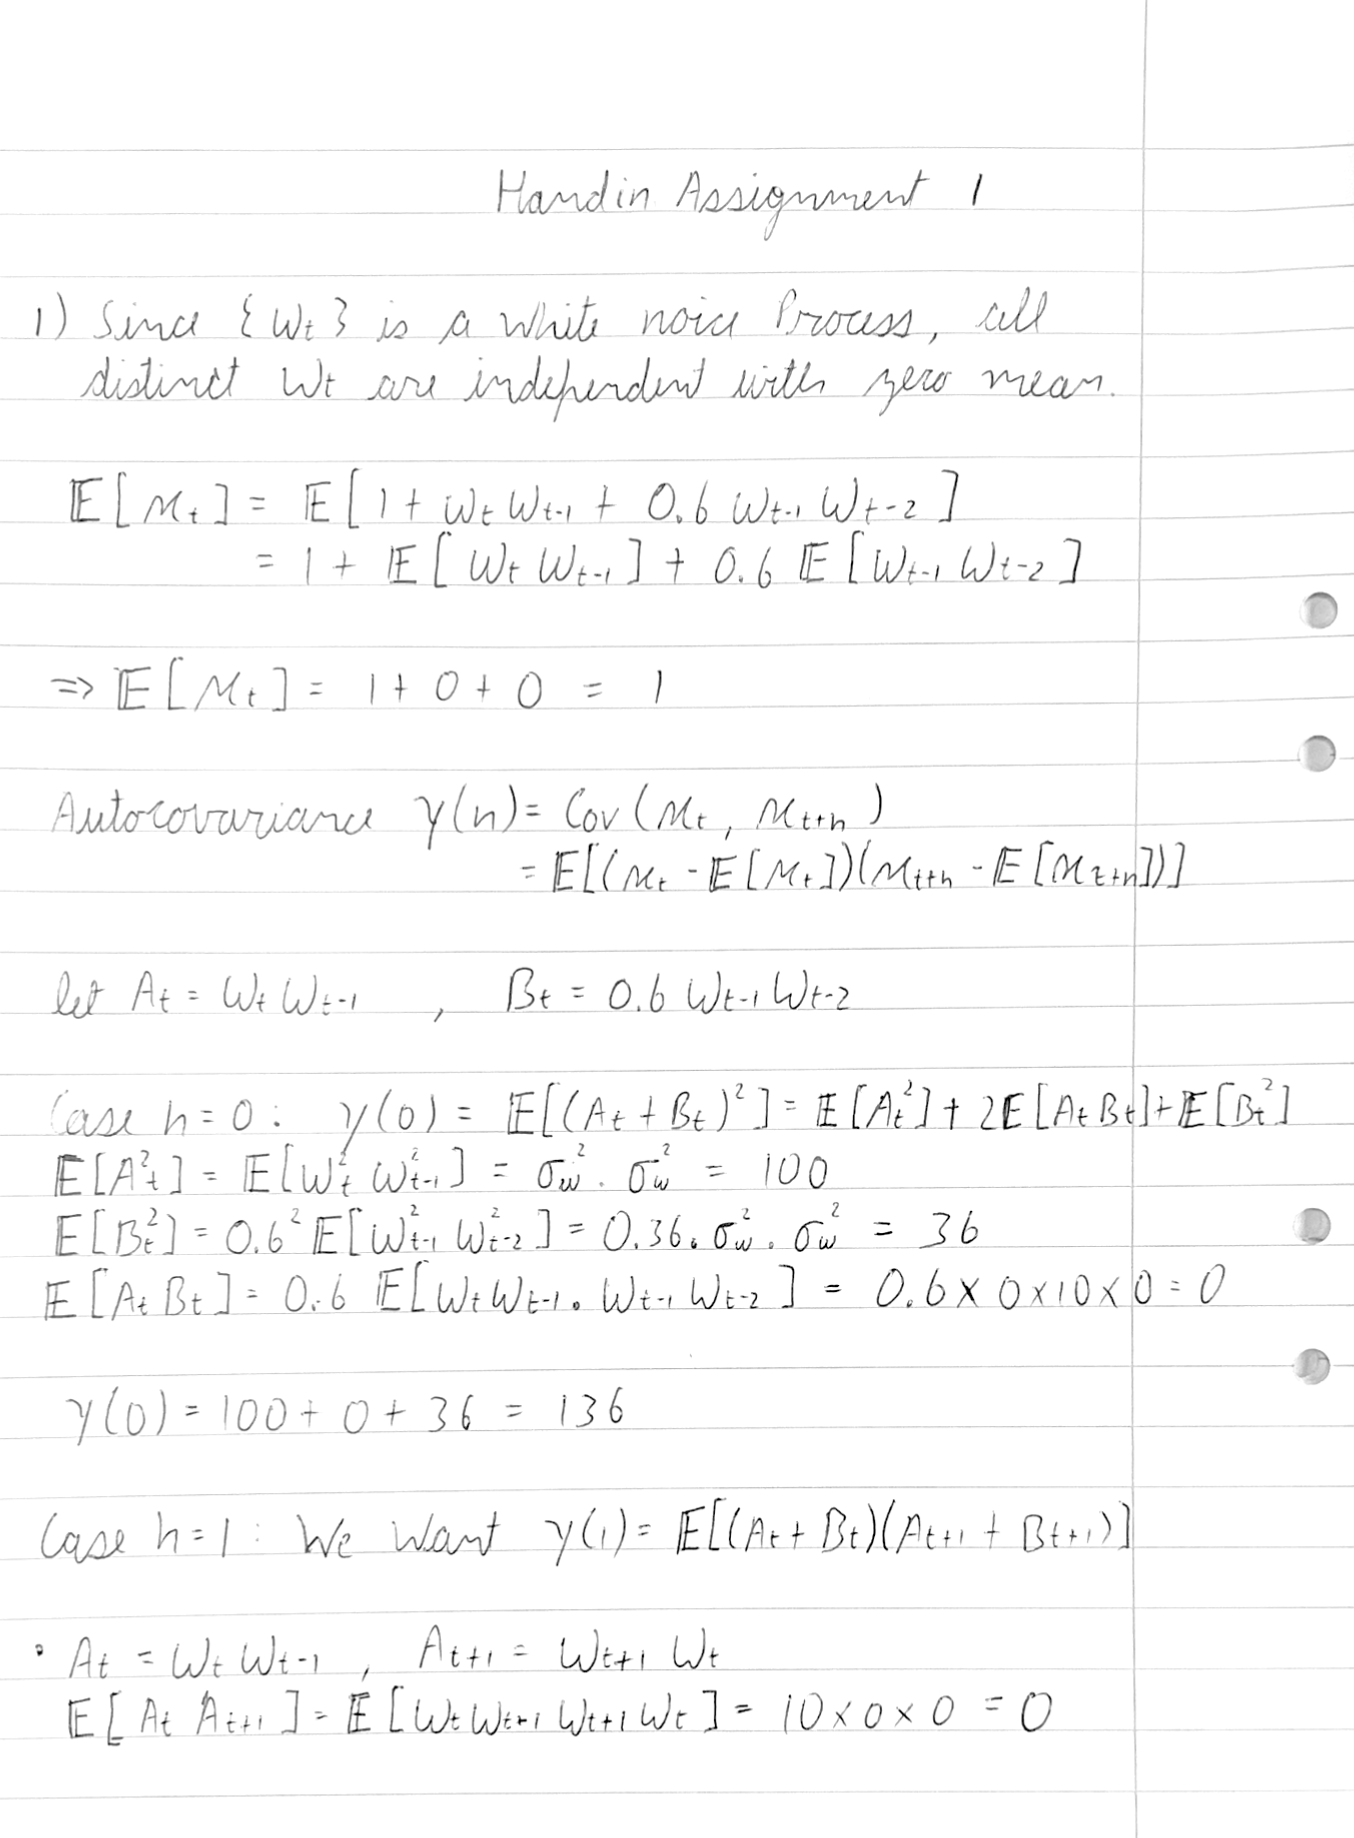
\includegraphics[width=1\textwidth]{ha-1_files/1-1.png}
        \label{fig:1}
    \end{figure}

    \begin{figure}[H]
        \centering
        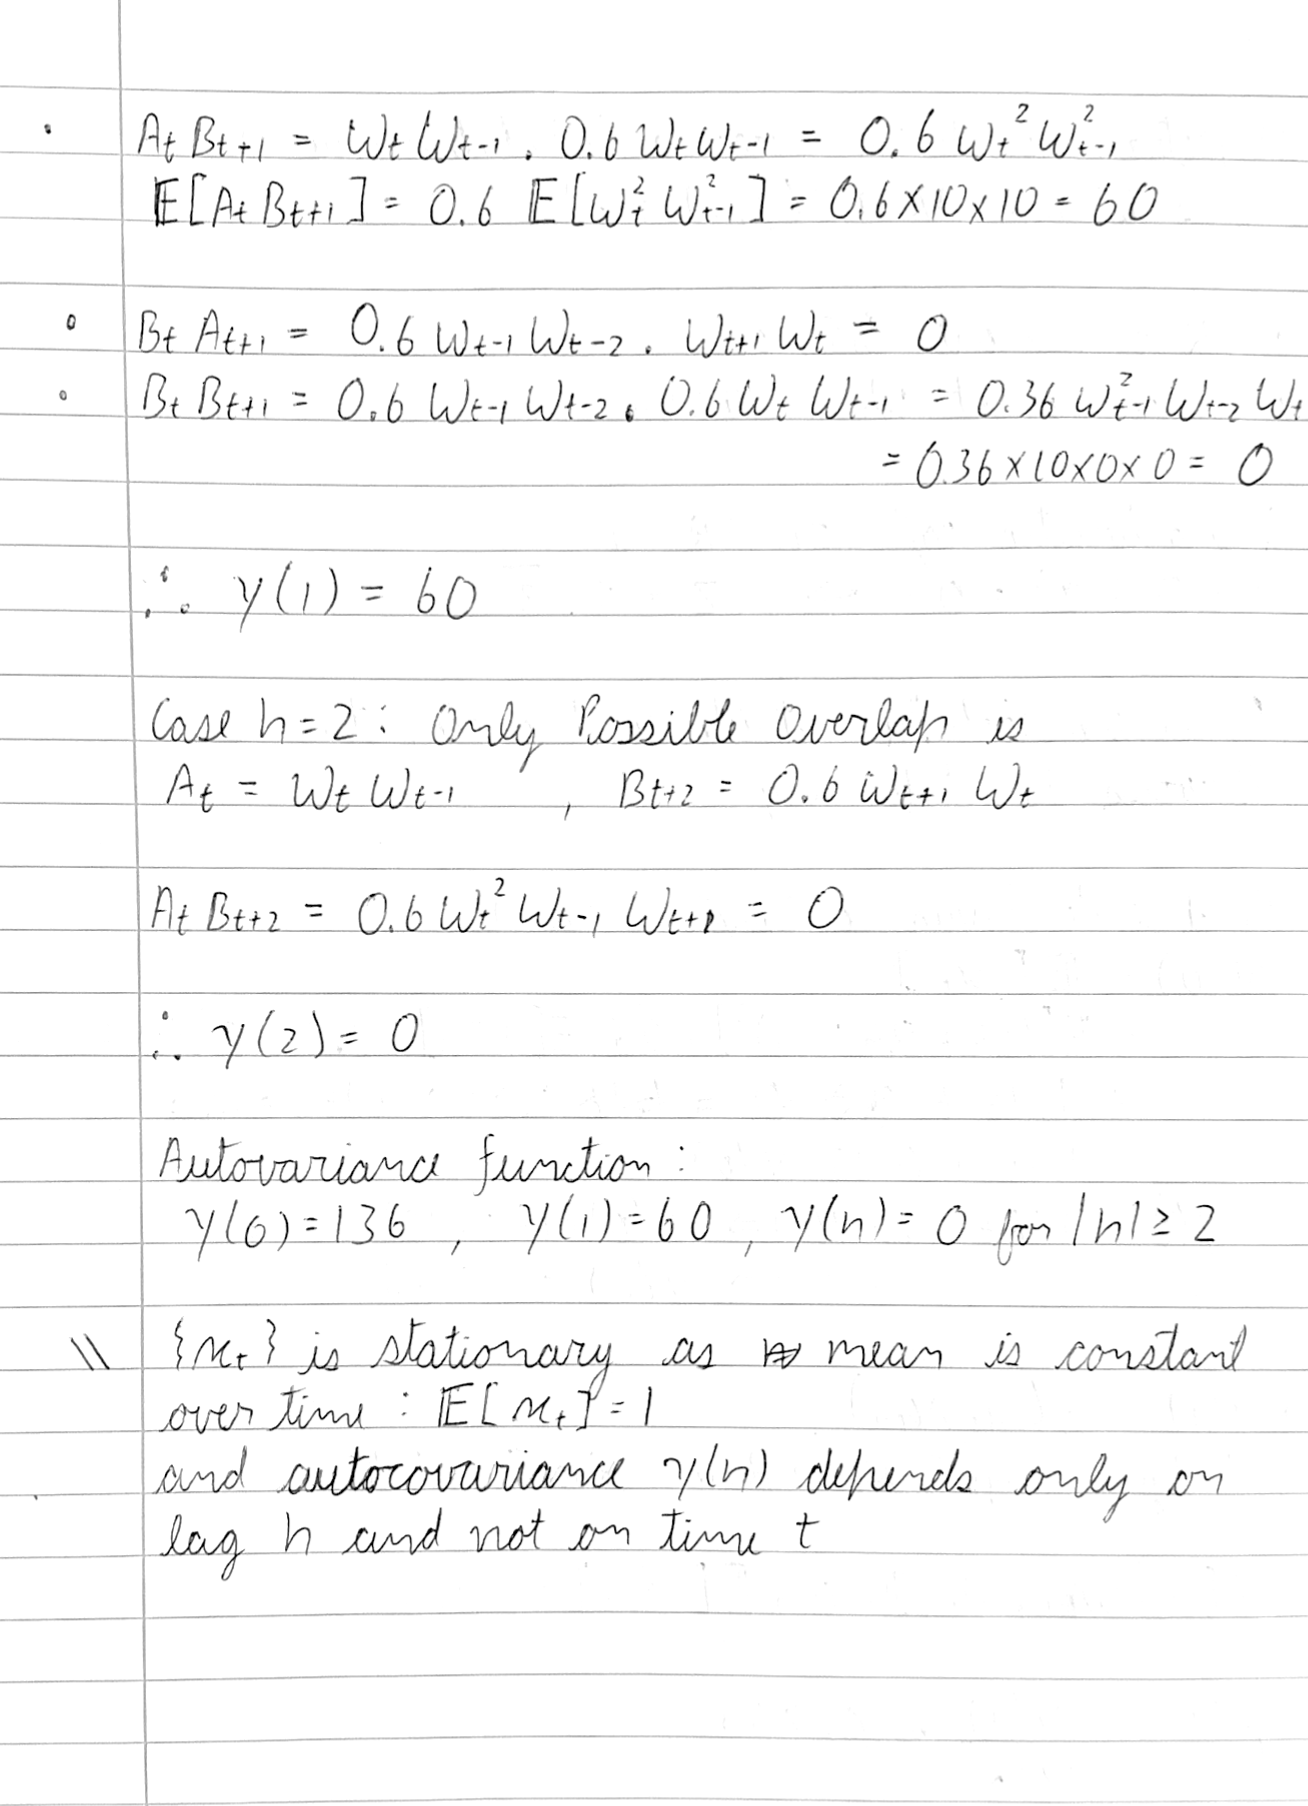
\includegraphics[width=1\textwidth]{ha-1_files/1-2.png}
        \label{fig:1-2}
    \end{figure}

    \newpage
    Task 2:    
    \begin{figure}[H]
        \centering
        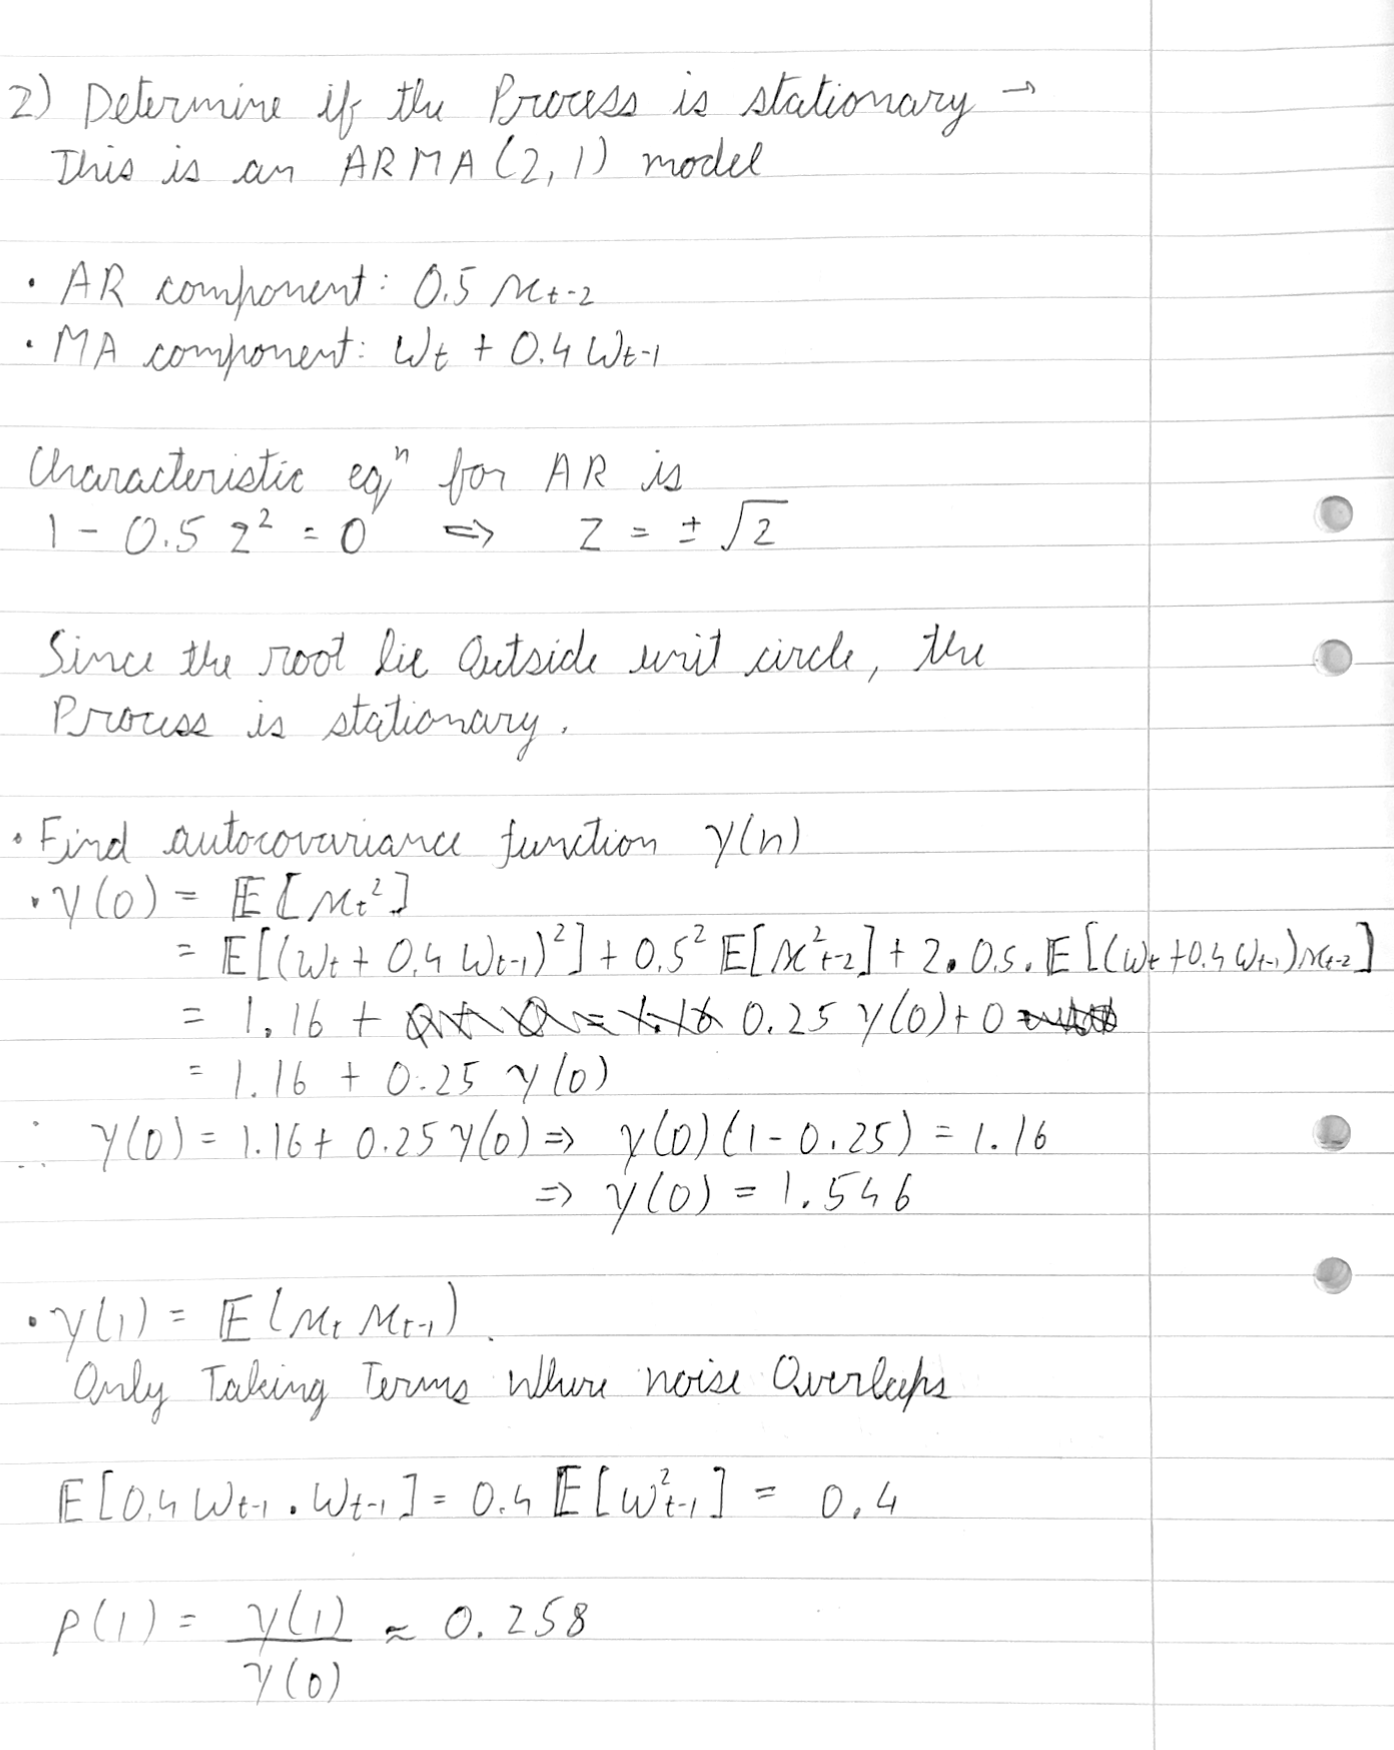
\includegraphics[width=1\textwidth]{ha-1_files/2-1.png}
        \label{fig:2}
    \end{figure}

    \begin{figure}[H]
        \centering
        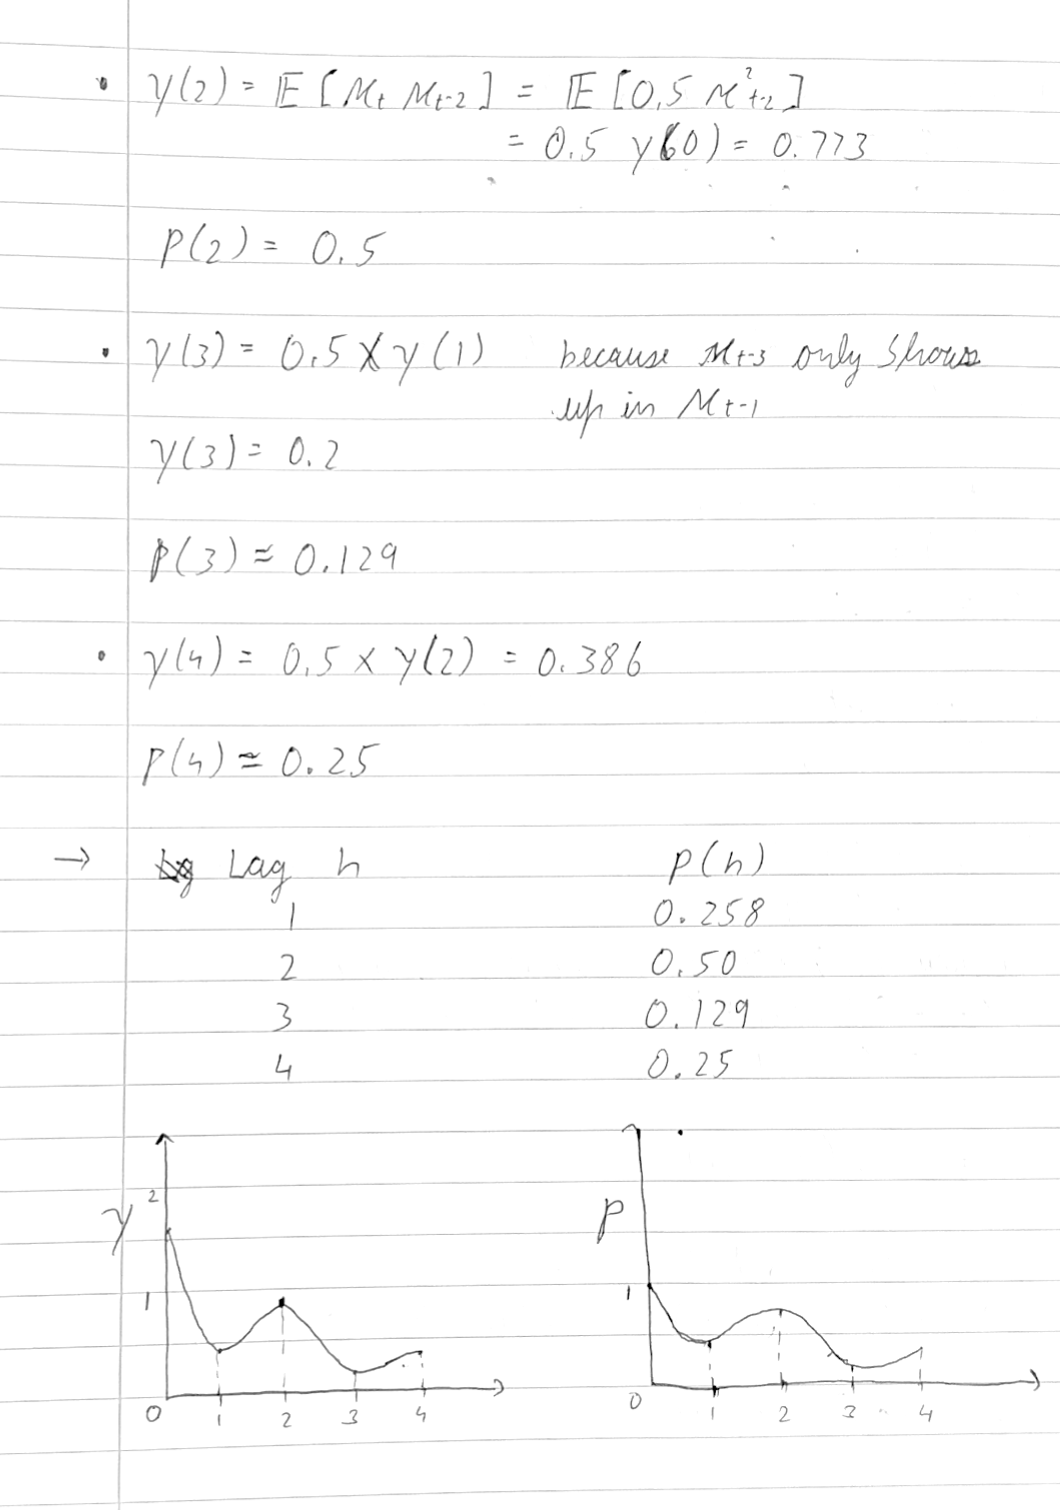
\includegraphics[width=1\textwidth]{ha-1_files/2-2.png}
        \label{fig:1-2}
    \end{figure}

    \newpage
    Task 3:    
    \begin{figure}[H]
        \centering
        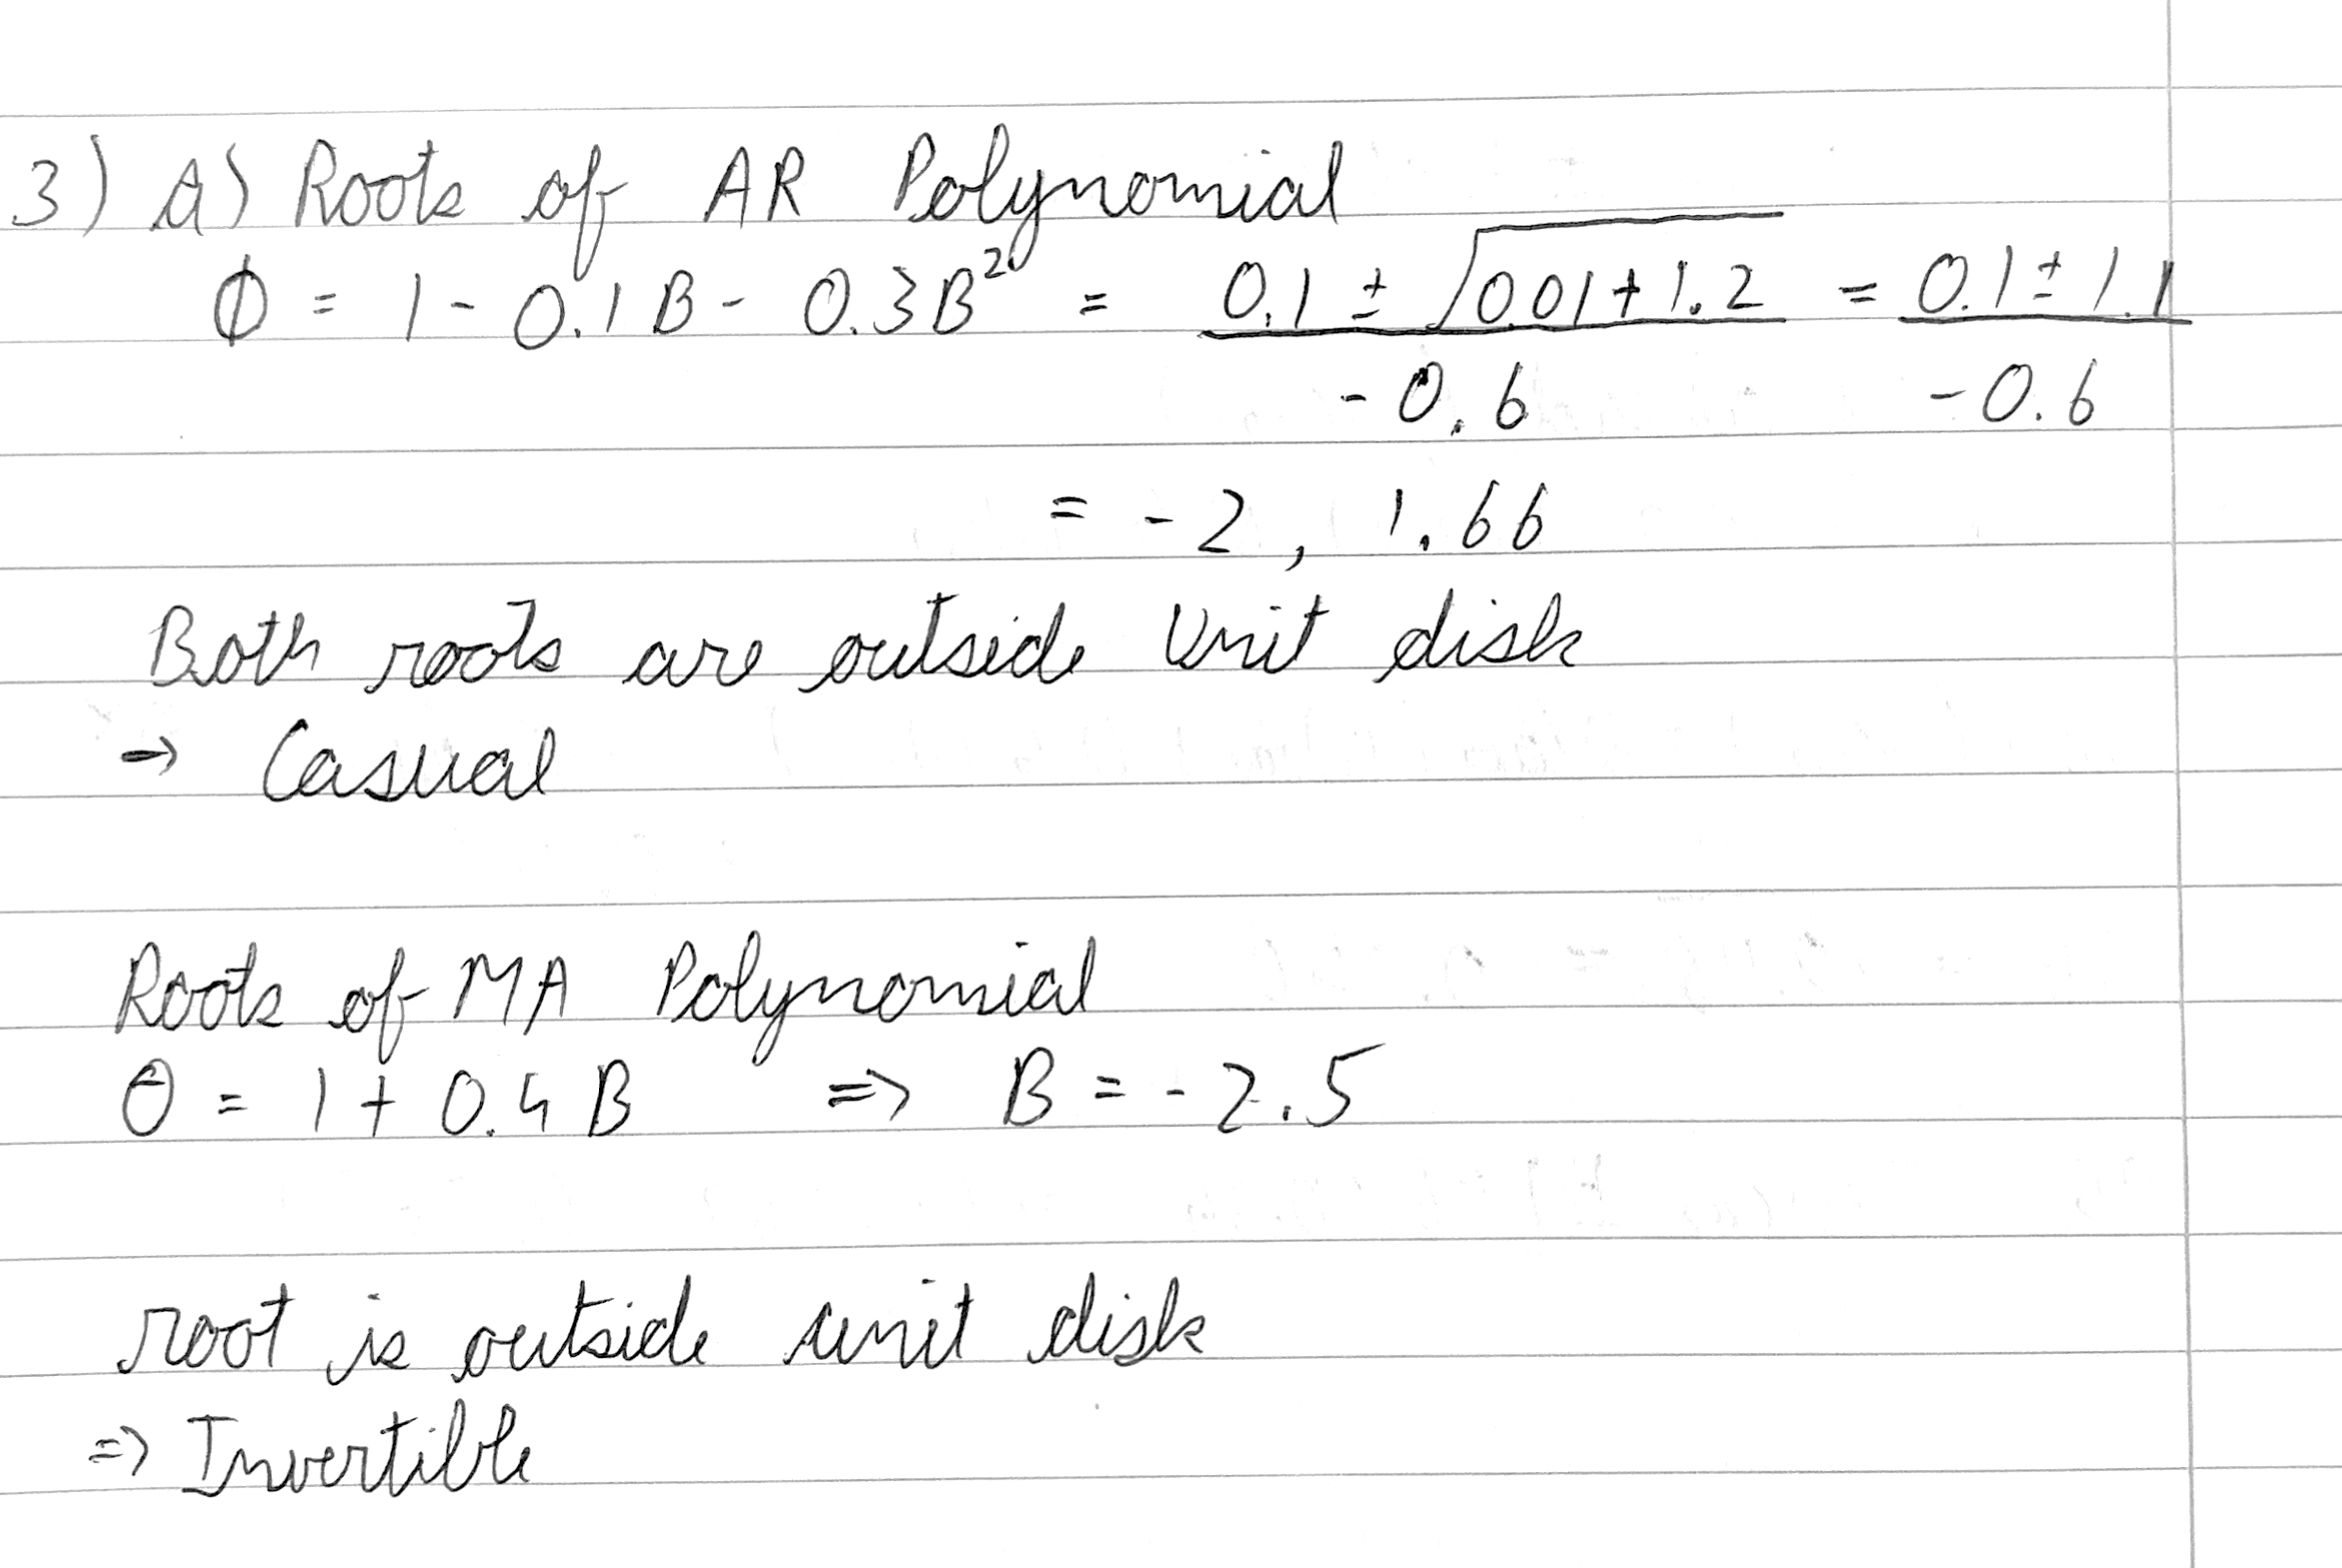
\includegraphics[width=1\textwidth]{ha-1_files/3-1.png}
        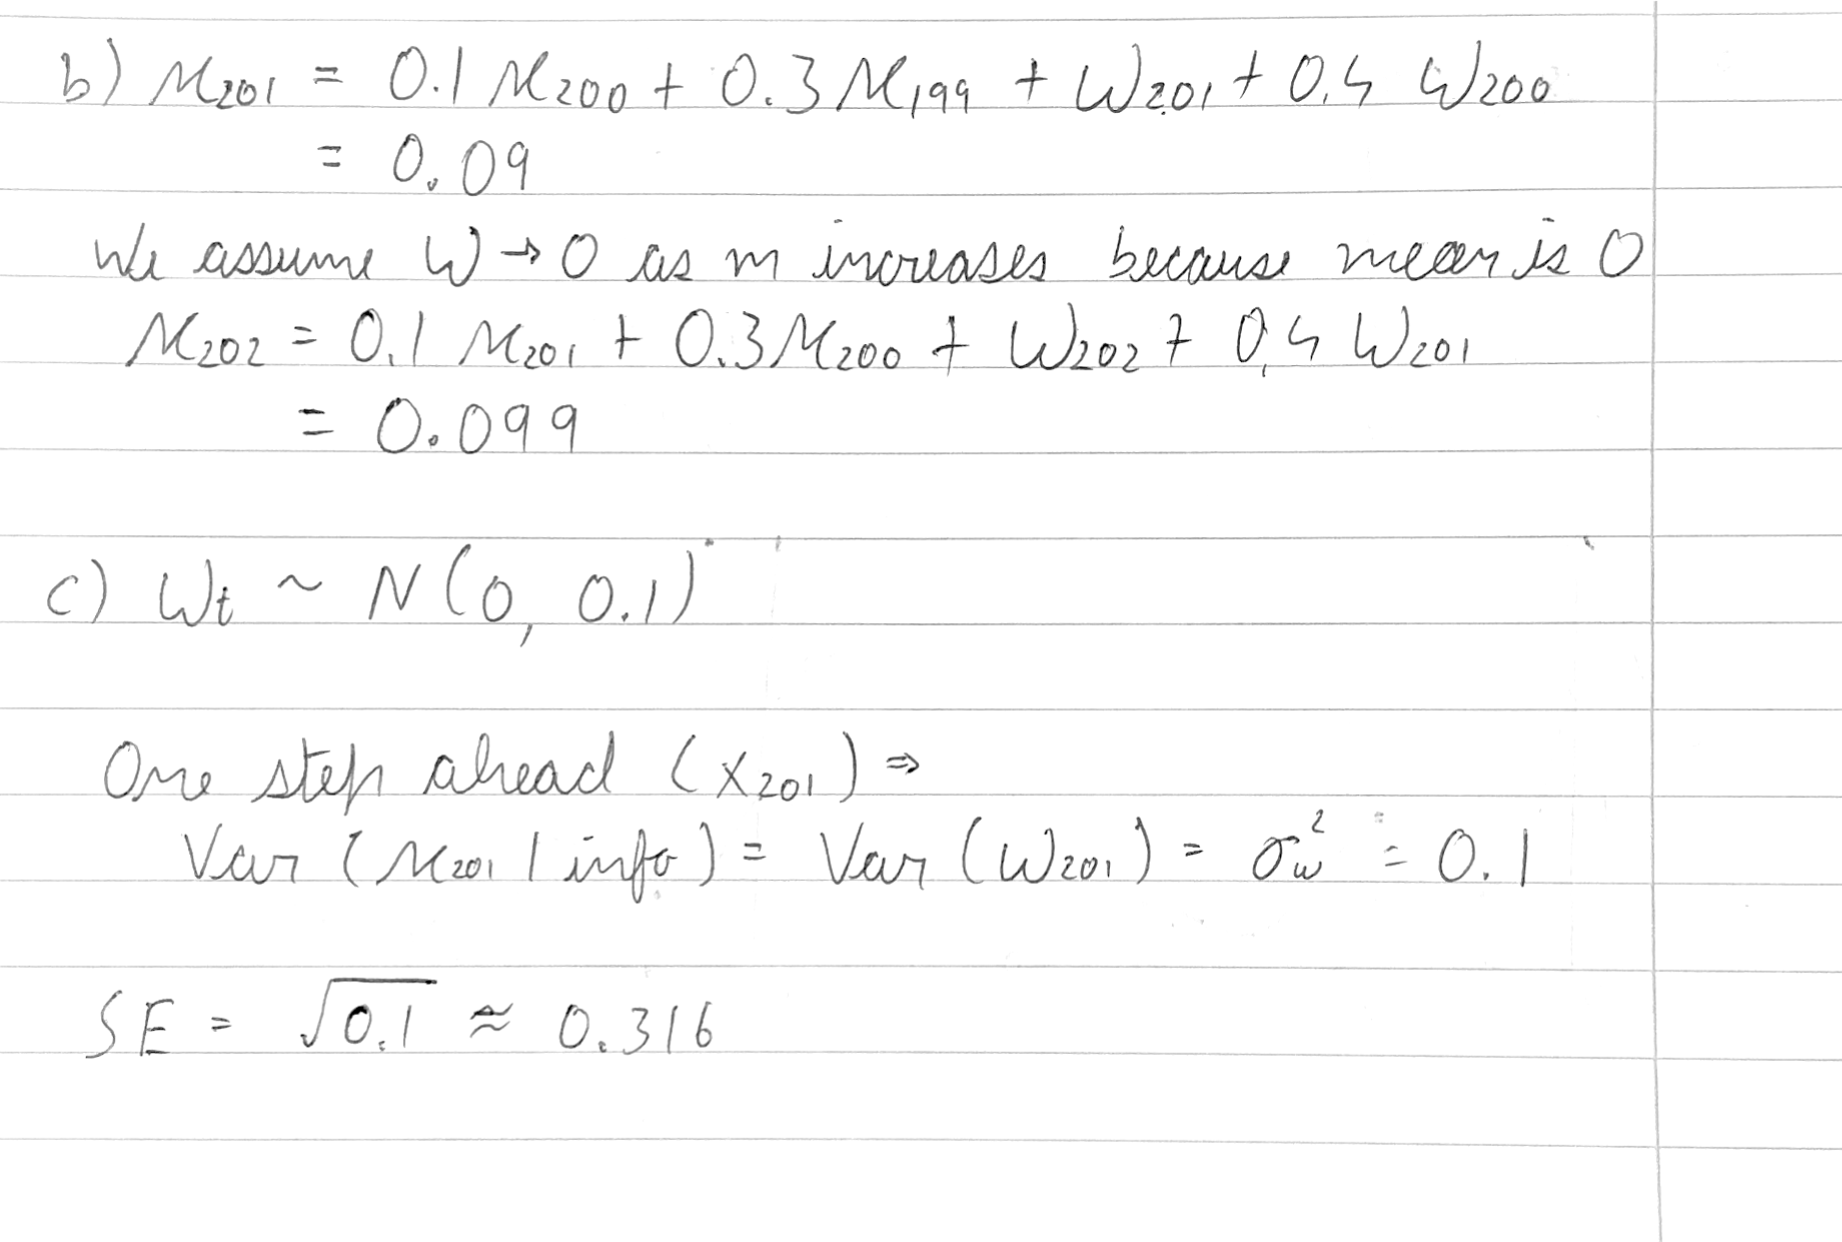
\includegraphics[width=1\textwidth]{ha-1_files/3-2.png}
        \label{fig:3}
    \end{figure}

    \newpage
    Task 4:

    The number of registered private cars in Sweden for the years 1977 until February 2025, monthly data, is given in the second column of the file carsmon.dat at Studium. 
    
    Find a suitable ARIMA (or SARIMA) model for these data, or a transformation thereof. Analyze the model residuals carefully, in order to make sure that the model provides a good description of the data. It might be a good idea to try transformations, like the logarithm.

    \_    
    \hrule

    Below is the time-series data plotted for the dataset of registered private cars from 1977-2025:

    \begin{figure}[H]
        \centering
        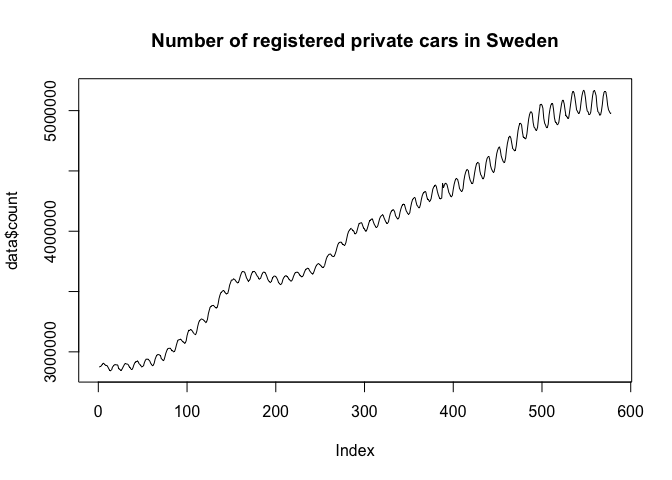
\includegraphics[width=0.6\textwidth]{ha-1_files/figure-markdown_strict/unnamed-chunk-1-1.png}
        \label{fig:f1}
    \end{figure}

    As the mean of the data with respect to time is changing, along with slight differences in the variance noticeable after around index 350, the data appears to be non-stationary initially. Upon applying a log transformation, to reduce the magnitude of the variance, and by applying a difference of lag=1, the graph looks like the following:

    \begin{figure}[H]
        \centering
        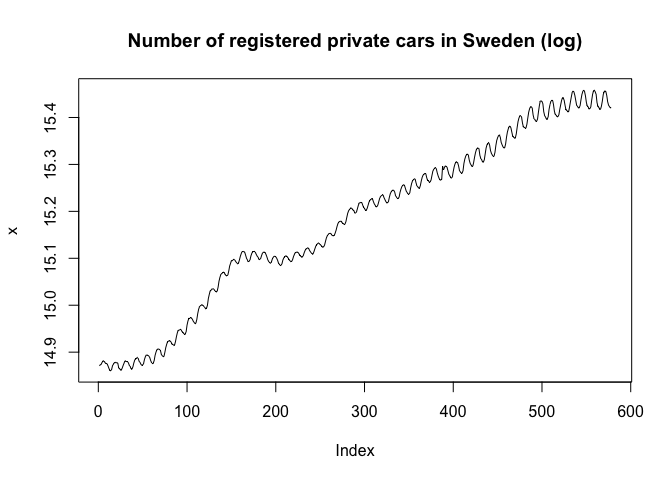
\includegraphics[width=0.7\textwidth]{ha-1_files/figure-markdown_strict/unnamed-chunk-1-2.png}
        \label{fig:f2}
    \end{figure}

    \begin{figure}[H]
        \centering
        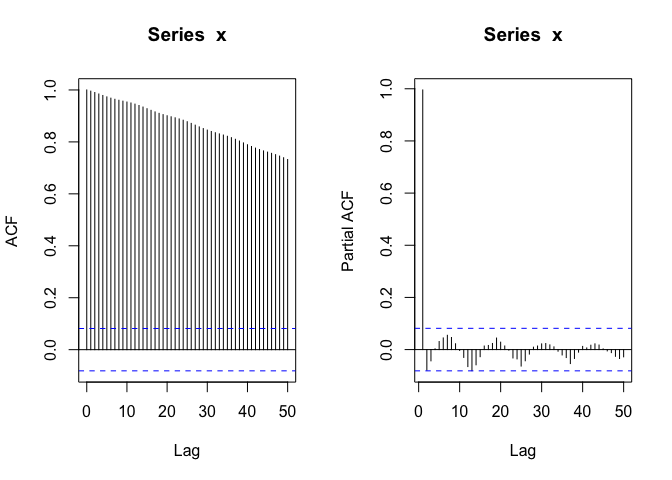
\includegraphics[width=0.8\textwidth]{ha-1_files/figure-markdown_strict/unnamed-chunk-1-3.png}
        \label{fig:f3}
    \end{figure}

    \begin{figure}[H]
        \centering
        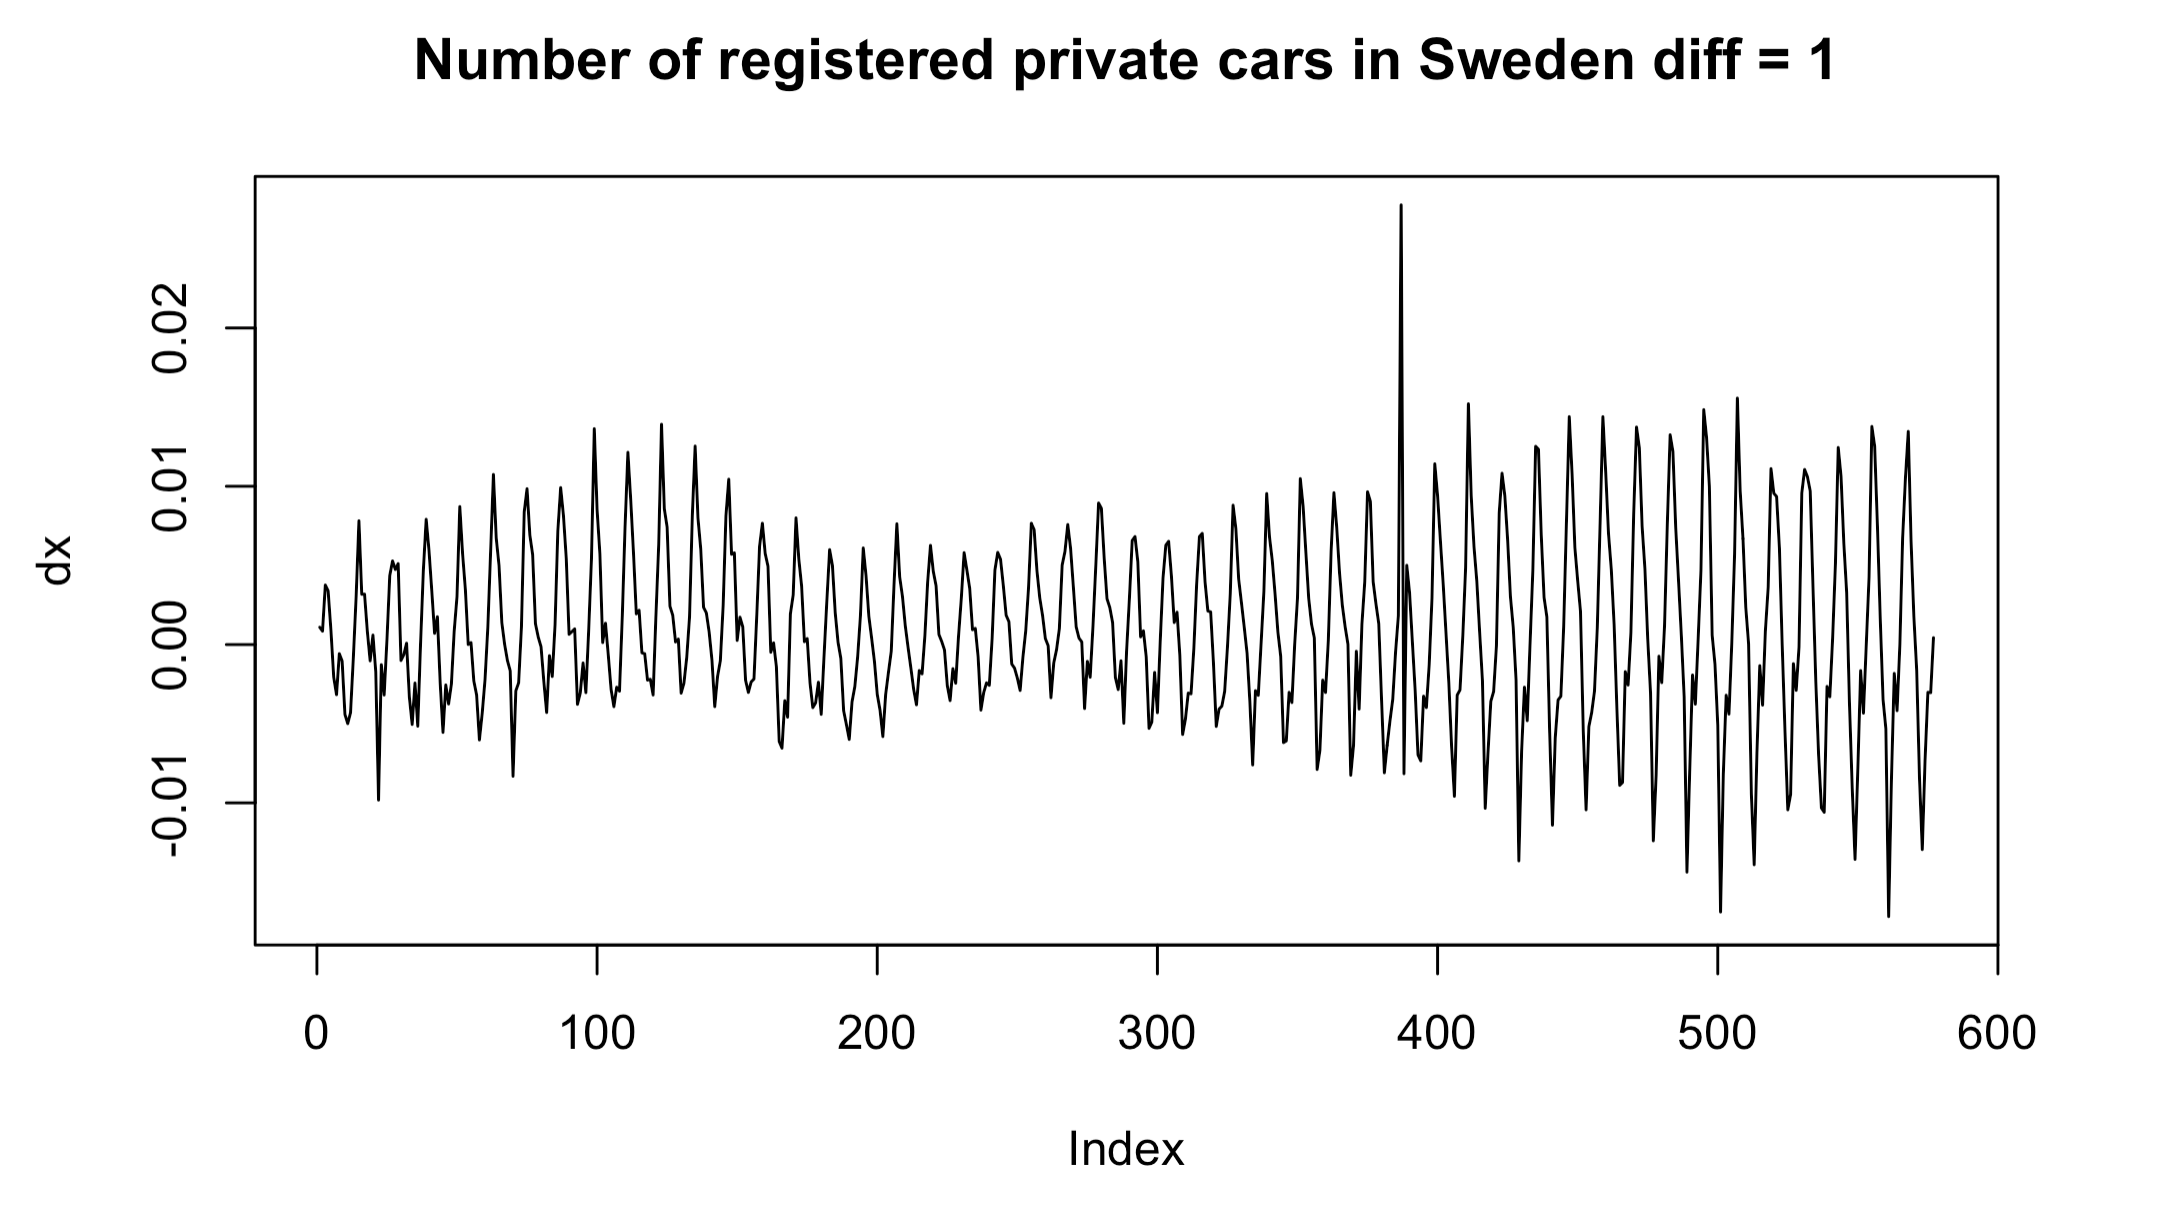
\includegraphics[width=0.8\textwidth]{ha-1_files/diff.png}
        \label{fig:f3}
    \end{figure}

    We now compute the autocorrelation (ACF) and partial autocorrelation (PACF) curves for the data, now that it is made to be more stationary. From the graphs, periodic peaks can be seen at lags 12, 24, 36 and so on, with a general slow decay. From the PACF, the noticeable peaks are present in lags up until 12, however, more information is yet to be derived. 

    \begin{figure}[H]
        \centering
        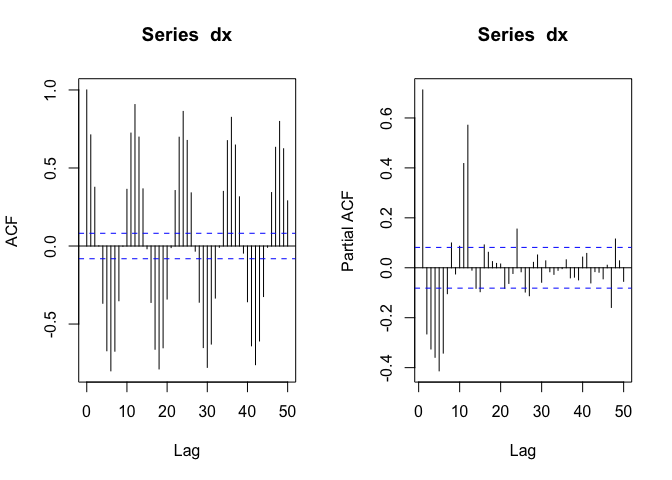
\includegraphics[width=0.8\textwidth]{ha-1_files/figure-markdown_strict/unnamed-chunk-2-2.png}
        \label{fig:f4}
    \end{figure}

    As some seasonal pattern is very likely present, we first try fitting an empty seasonal model, where the period is set to 12.

    \[\text{ARIMA}(0,1,0).(0,1,0)_{12}\]

    \begin{figure}[H]
        \centering
        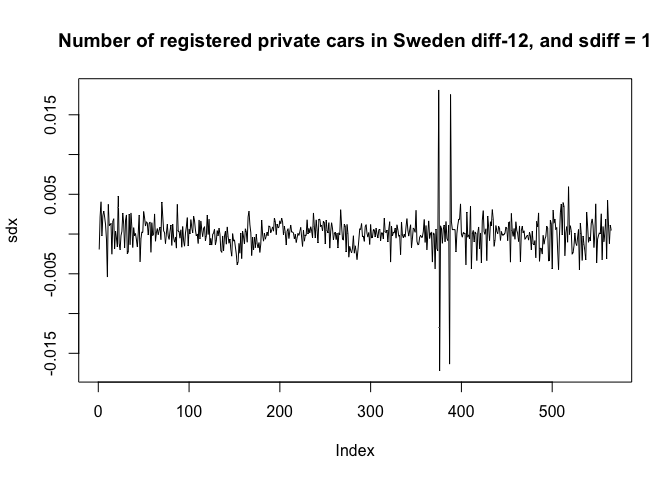
\includegraphics[width=0.4\textwidth]{ha-1_files/figure-markdown_strict/unnamed-chunk-3-1.png}
        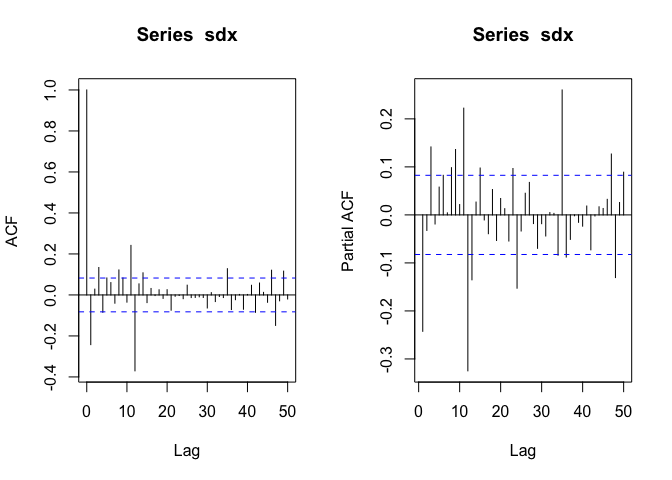
\includegraphics[width=0.4\textwidth]{ha-1_files/figure-markdown_strict/unnamed-chunk-3-2.png}
        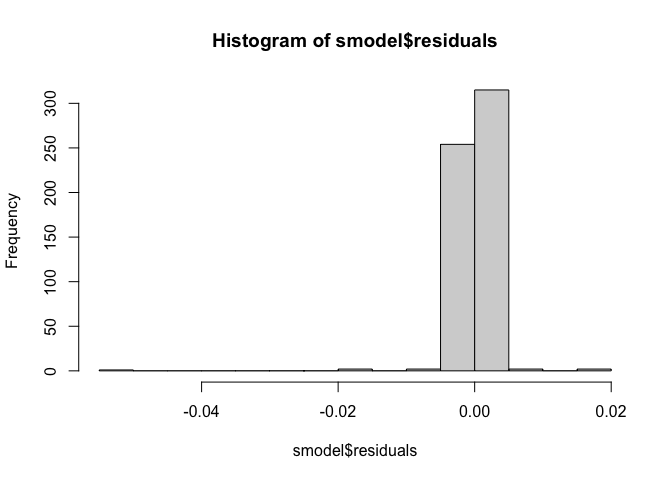
\includegraphics[width=0.4\textwidth]{ha-1_files/figure-markdown_strict/unnamed-chunk-3-3.png}
        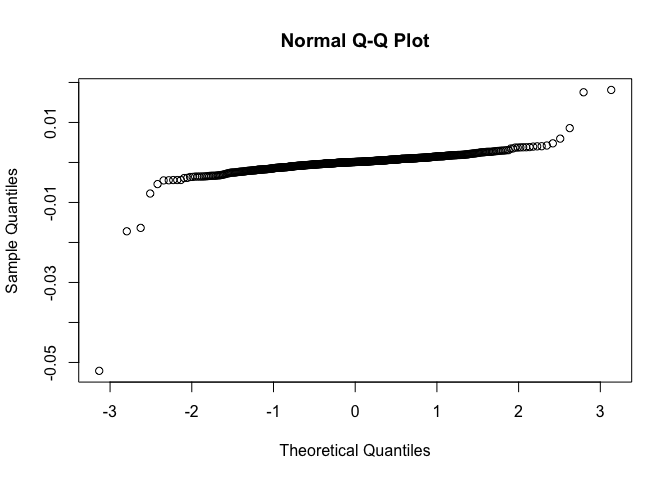
\includegraphics[width=0.4\textwidth]{ha-1_files/figure-markdown_strict/unnamed-chunk-3-4.png}
        \label{fig:f5}
    \end{figure}

    \begin{figure}[H]
        \centering
        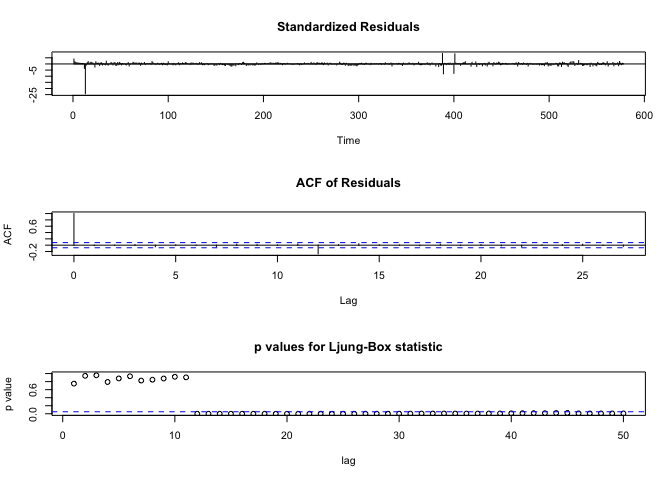
\includegraphics[width=0.8\textwidth]{ha-1_files/figure-markdown_strict/unnamed-chunk-3-5.png}
        \label{fig:f6}
    \end{figure}

    \textbf{Description of the p-values, and relevant statistics:} From the empty SARIMA model, log likelihood was calculated as 2670.76 and the Akaike Information Criterion (aic) was -5339.52. 

    A general SARIMA model looks like the following (with difference kept constant to 1, as the stationarity aspect was achieved, and over-differencing may negatively impact the results):
    \[\text{SARIMA}(p,1,q).(P,1,Q)_{12}\]

    The main signs to find the model best fitting to the time-series data are i) \textit{inspecting the standardized residuals, as well as their ACF/PACF} to see if white-noise like behaviour is shown, ii) \textit{Ljung-Box Statistic p-values} and their behvaiour with increasing lags (not going below the error bound for longer lags), and iii) the AIC. 

    A grid-search based approach was done, where p, q (for the non-seasonal component), and P, Q (seasonal component) were varied from range of 0 to 4. The first iteration gave the benchmark empty seasonal model described earlier. 
    
    In the first few iterations, an example is $\text{SARIMA}(0,1,0).(1,1,0)_{12}$, which had good p-values for later lags than 12, above the acceptance threshold (seasonal AR(1)). By means of inspection after the received ACF/PACF plots, 15 models with significant p-values in the Ljung-Box plots were:

    \vspace{-20pt}

    \begin{itemize}
        \item $\text{SARIMA}(0,1,0).(1,1,0)_{12}$, $\text{SARIMA}(0,1,0).(2,1,0)_{12}$
        \item $\text{SARIMA}(3,1,3).(0,1,1)_{12}$, $\text{SARIMA}(3,1,3).(0,1,2)_{12}$, $\text{SARIMA}(3,1,3).(0,1,3)_{12}$, \\ $\text{SARIMA}(3,1,3).(0,1,4)_{12}$
        \item $\text{SARIMA}(3,1,3).(1,1,1)_{12}$, $\text{SARIMA}(3,1,3).(1,1,2)_{12}$, $\text{SARIMA}(3,1,3).(1,1,3)_{12}$, \\ $\text{SARIMA}(3,1,3).(1,1,4)_{12}$
        \item $\text{SARIMA}(3,1,3).(2,1,1)_{12}$, $\text{SARIMA}(3,1,3).(2,1,2)_{12}$, $\text{SARIMA}(3,1,3).(2,1,3)_{12}$
        \item $\text{SARIMA}(3,1,3).(3,1,0)_{12}$, $\text{SARIMA}(3,1,3).(3,1,1)_{12}$
    \end{itemize}

    An example of a model with p-values above the confidence threshold for longer lags from h=12 is shown here:

    \begin{figure}[H]
        \centering
        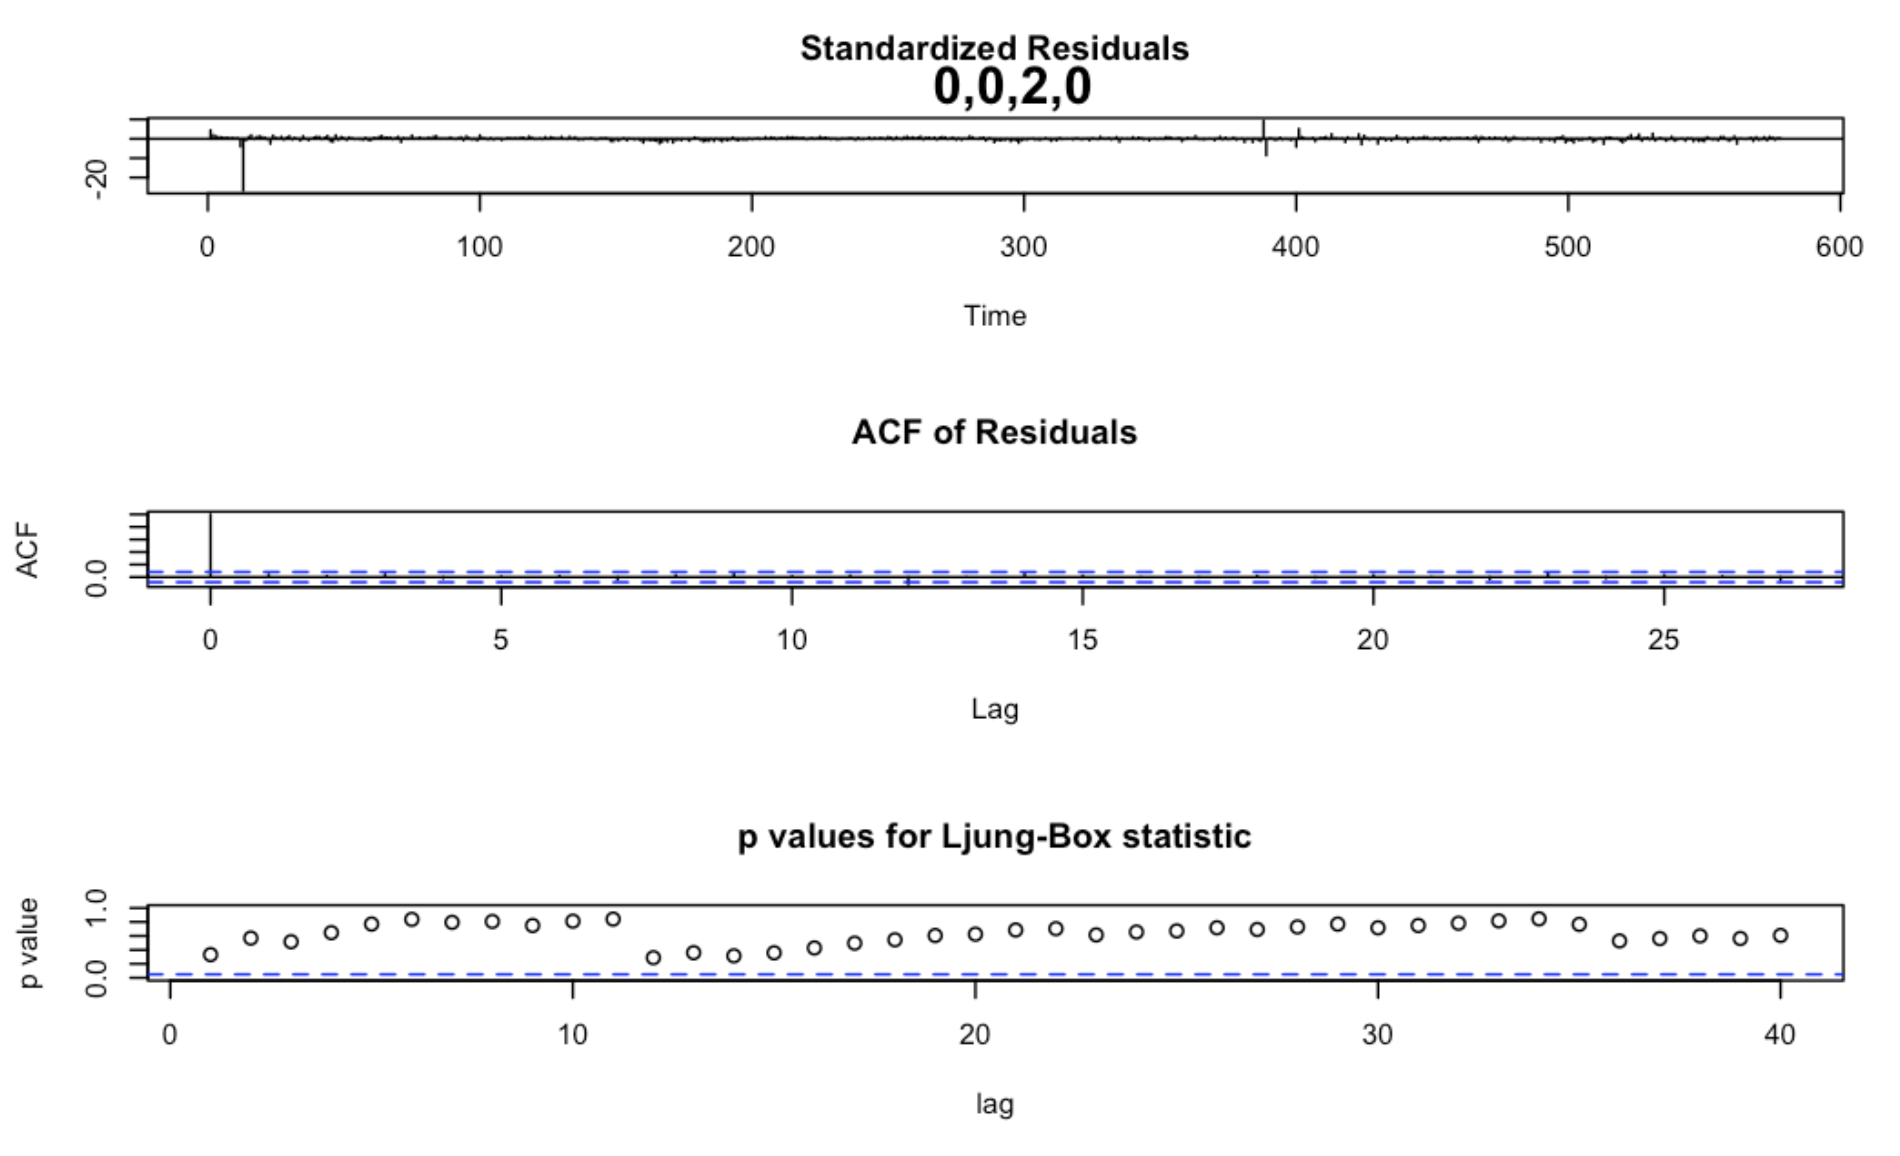
\includegraphics[width=0.8\textwidth]{ha-1_files/figure-markdown_strict/0-0-2-0.png}
        \label{fig:f7}
    \end{figure}

    The top-3 smallest AICs from all of the observed good p-value SARIMA models, are marked below:

    \begin{itemize}
        \item ... $\text{SARIMA}(0,1,0).(2,1,0)_{12}$ -5441.355
        \item $\text{SARIMA}(3,1,3).(0,1,1)_{12}$ \textbf{-5532.681}, $\text{SARIMA}(3,1,3).(0,1,2)_{12}$ \textbf{-5530.727}, \\ $\text{SARIMA}(3,1,3).(0,1,3)_{12}$ -5528.845, $\text{SARIMA}(3,1,3).(0,1,4)_{12}$ -5528.377
        \item $\text{SARIMA}(3,1,3).(1,1,1)_{12}$ \textbf{-5530.729}, $\text{SARIMA}(3,1,3).(1,1,2)_{12}$ -5528.817, \\ $\text{SARIMA}(3,1,3).(1,1,3)_{12}$ -5527.005, $\text{SARIMA}(3,1,3).(1,1,4)_{12}$ -5526.928
        \item ...
    \end{itemize}

    Hence, a SARIMA model to fit the registered cars time-series dataset chosen, based on the achieved AICs, and manual inspection of the Ljung-Box Statistics, and the residuals having a random, white-noise like behaviour, apart from small outliers, is $\text{SARIMA}(3,1,3).(0,1,1)_{12}$ (AIC: \textbf{-5532.681}). 

    \vspace{-10pt}
    \begin{figure}[H]
        \centering
        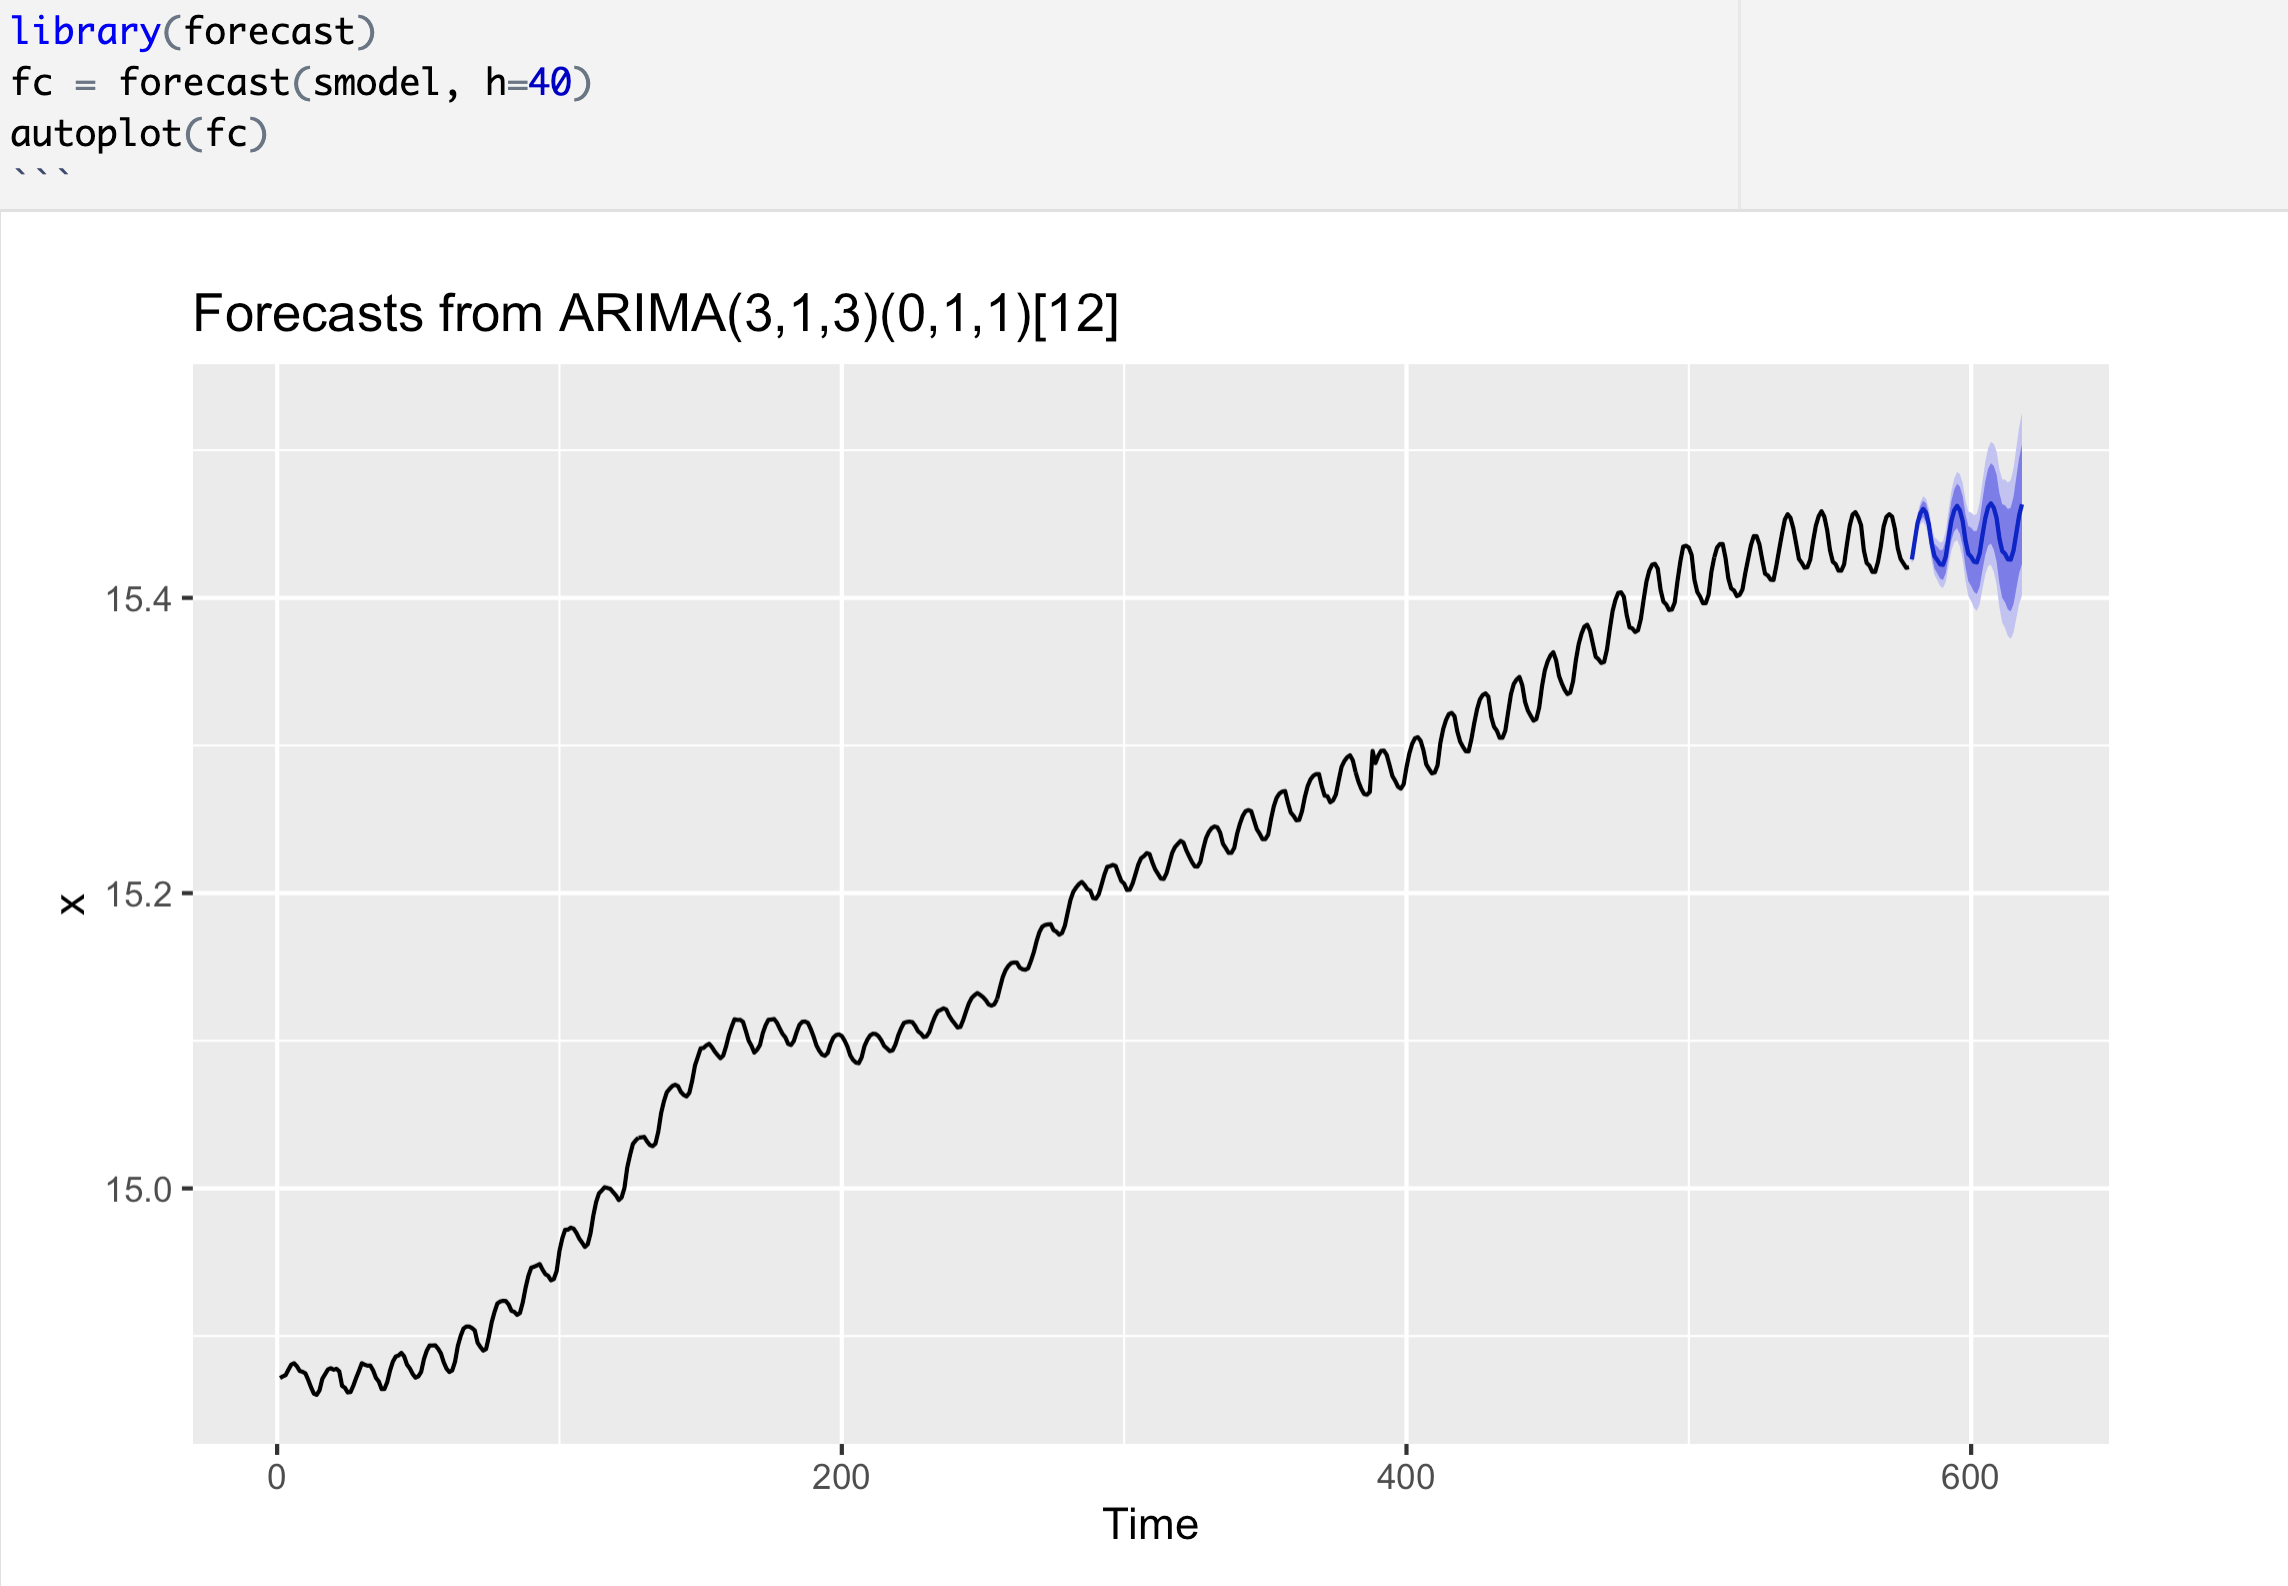
\includegraphics[width=0.6\textwidth]{ha-1_files/figure-markdown_strict/forecast.png}
        \label{fig:forecast}
    \end{figure}

    \newpage
    \textbf{Detailed plots of the top-3 lowest-AIC SARIMA models fitted, AND significant p-values:}

    \begin{figure}[H]
        \centering
        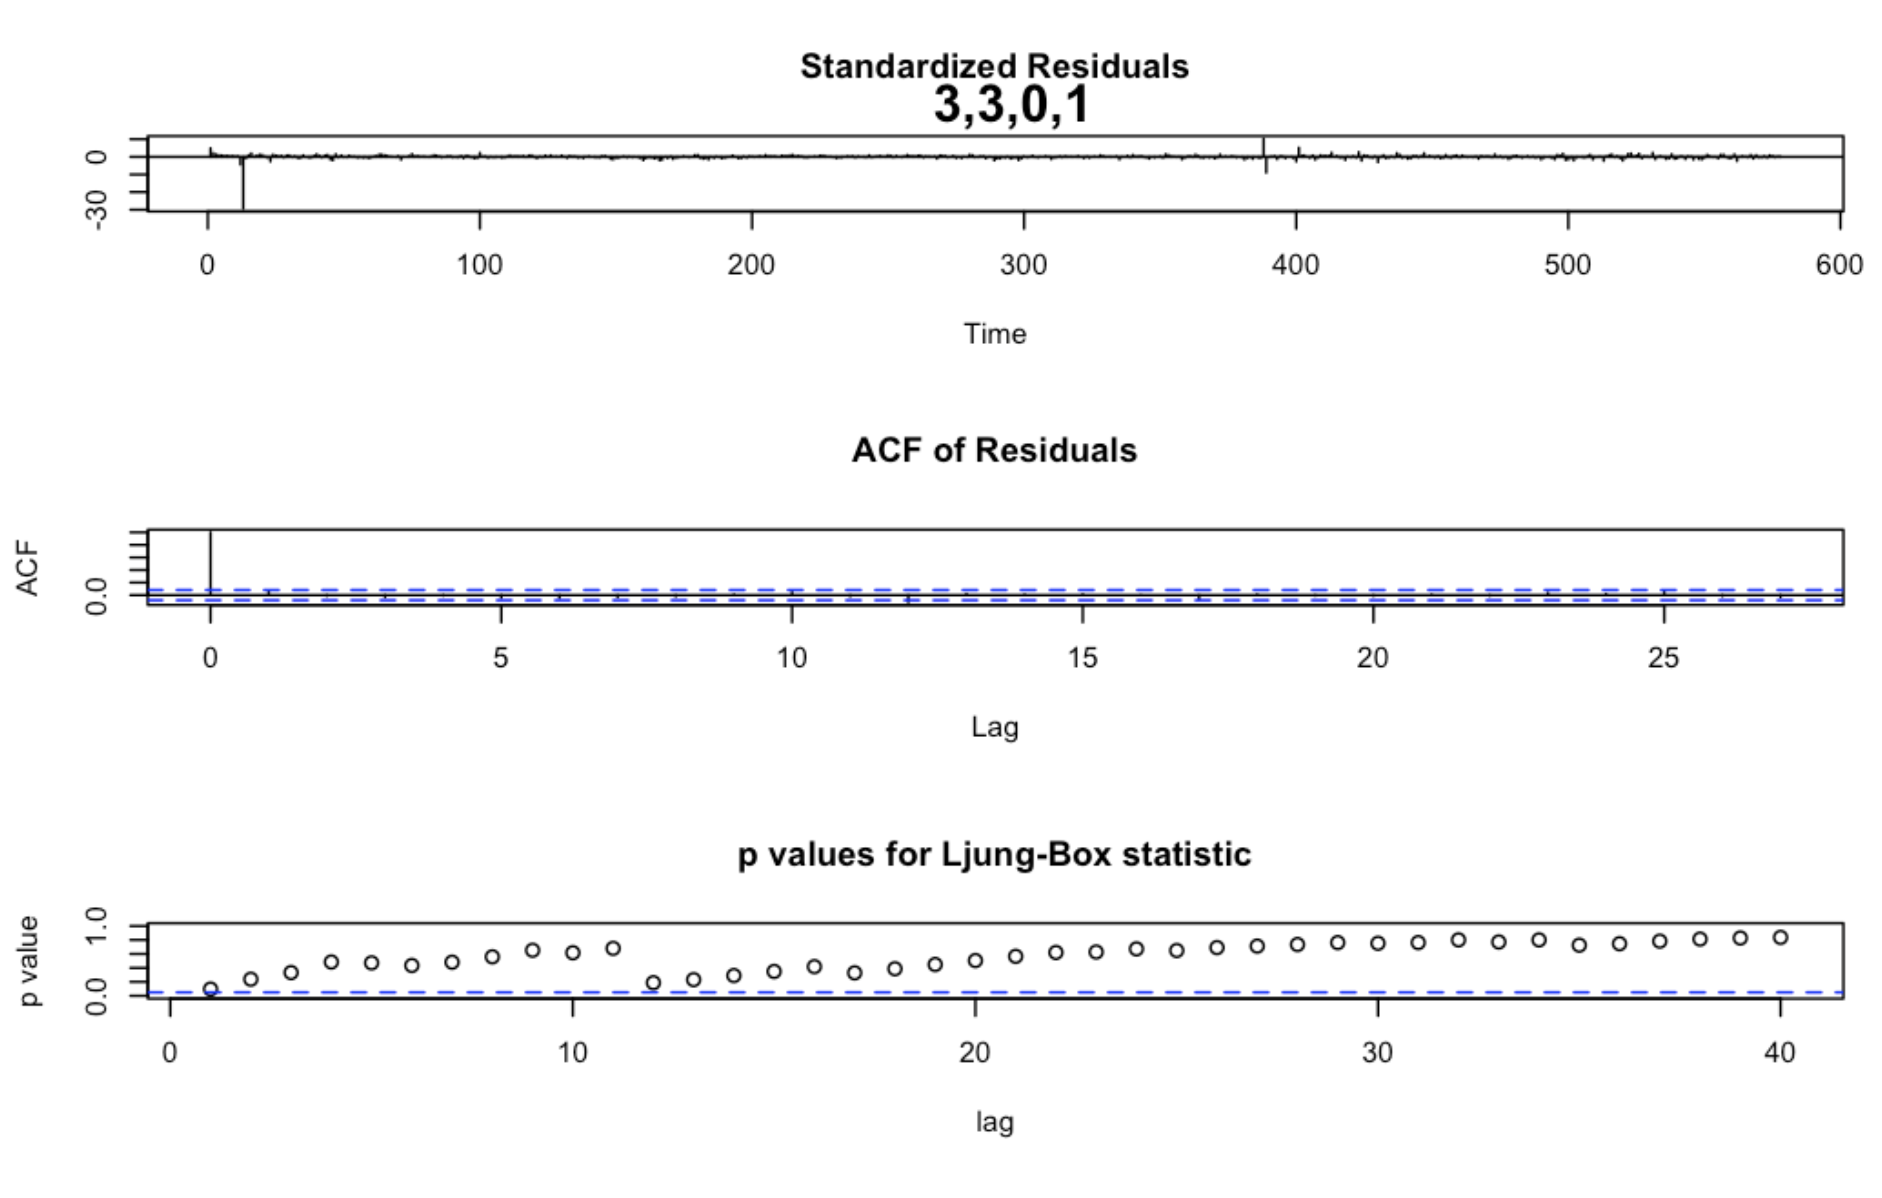
\includegraphics[width=0.7\textwidth]{ha-1_files/figure-markdown_strict/3-3-0-1.png}
        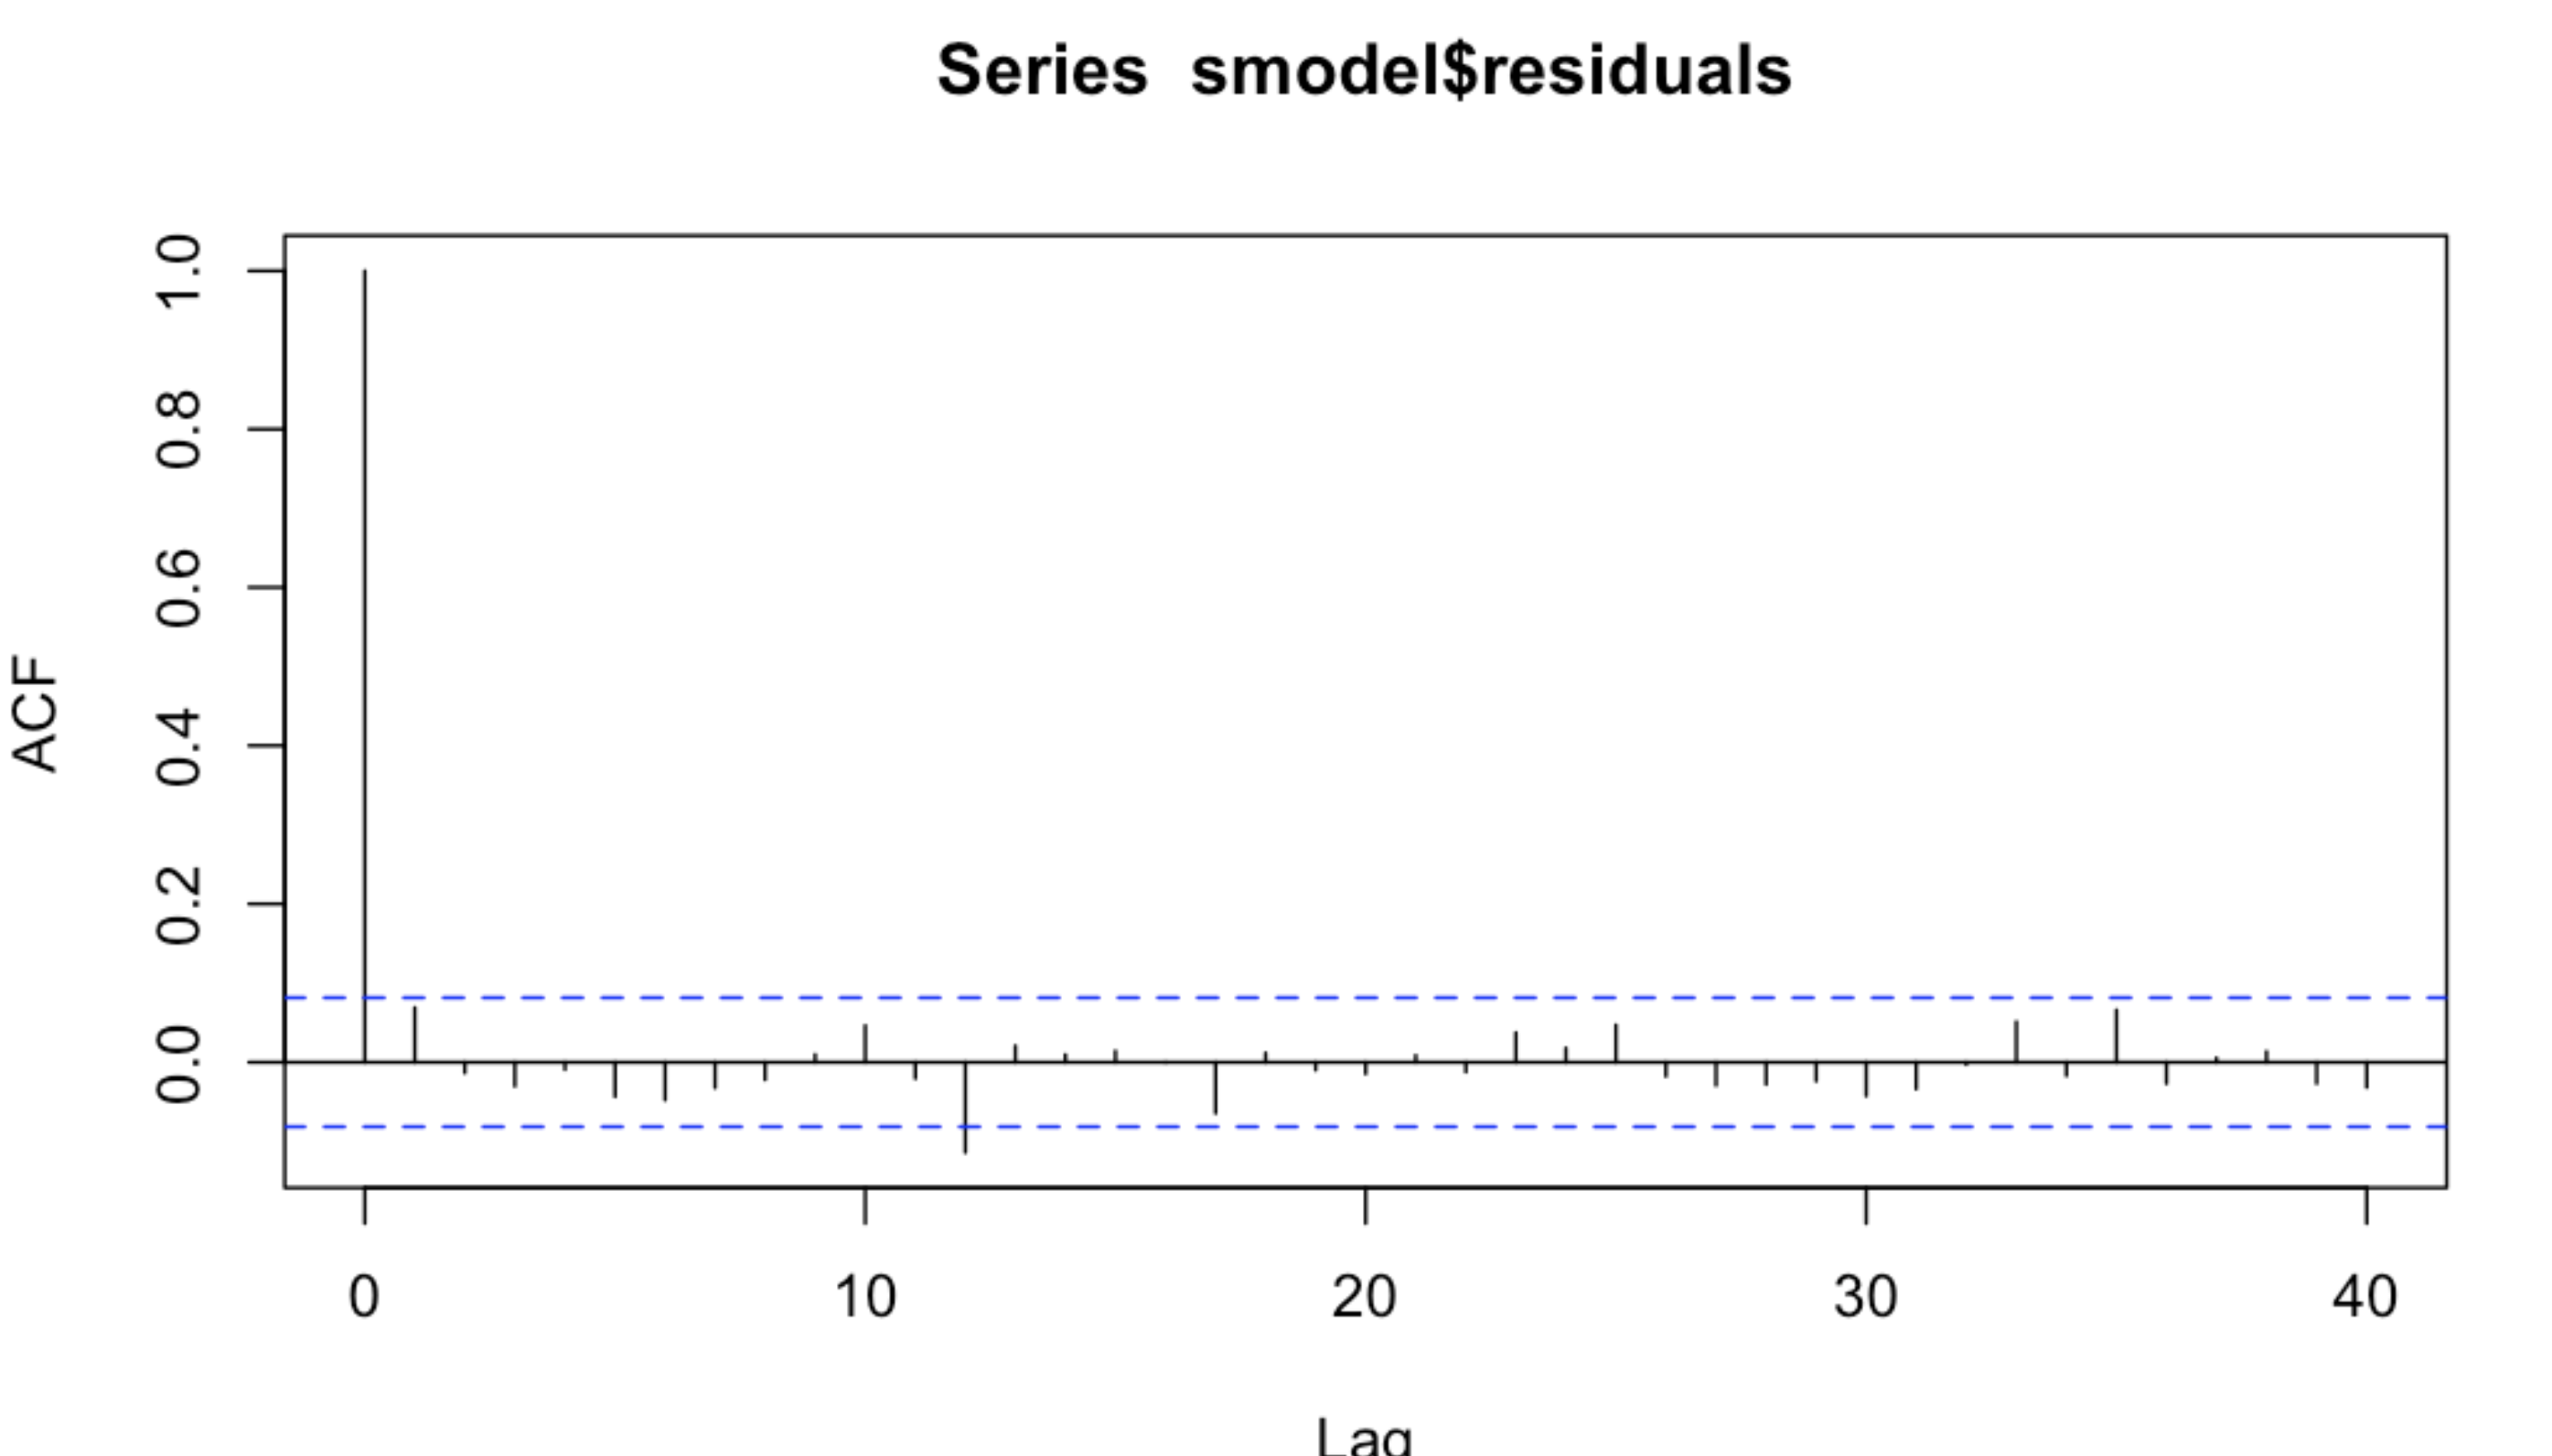
\includegraphics[width=0.7\textwidth]{ha-1_files/figure-markdown_strict/3-3-0-1.1.png}
        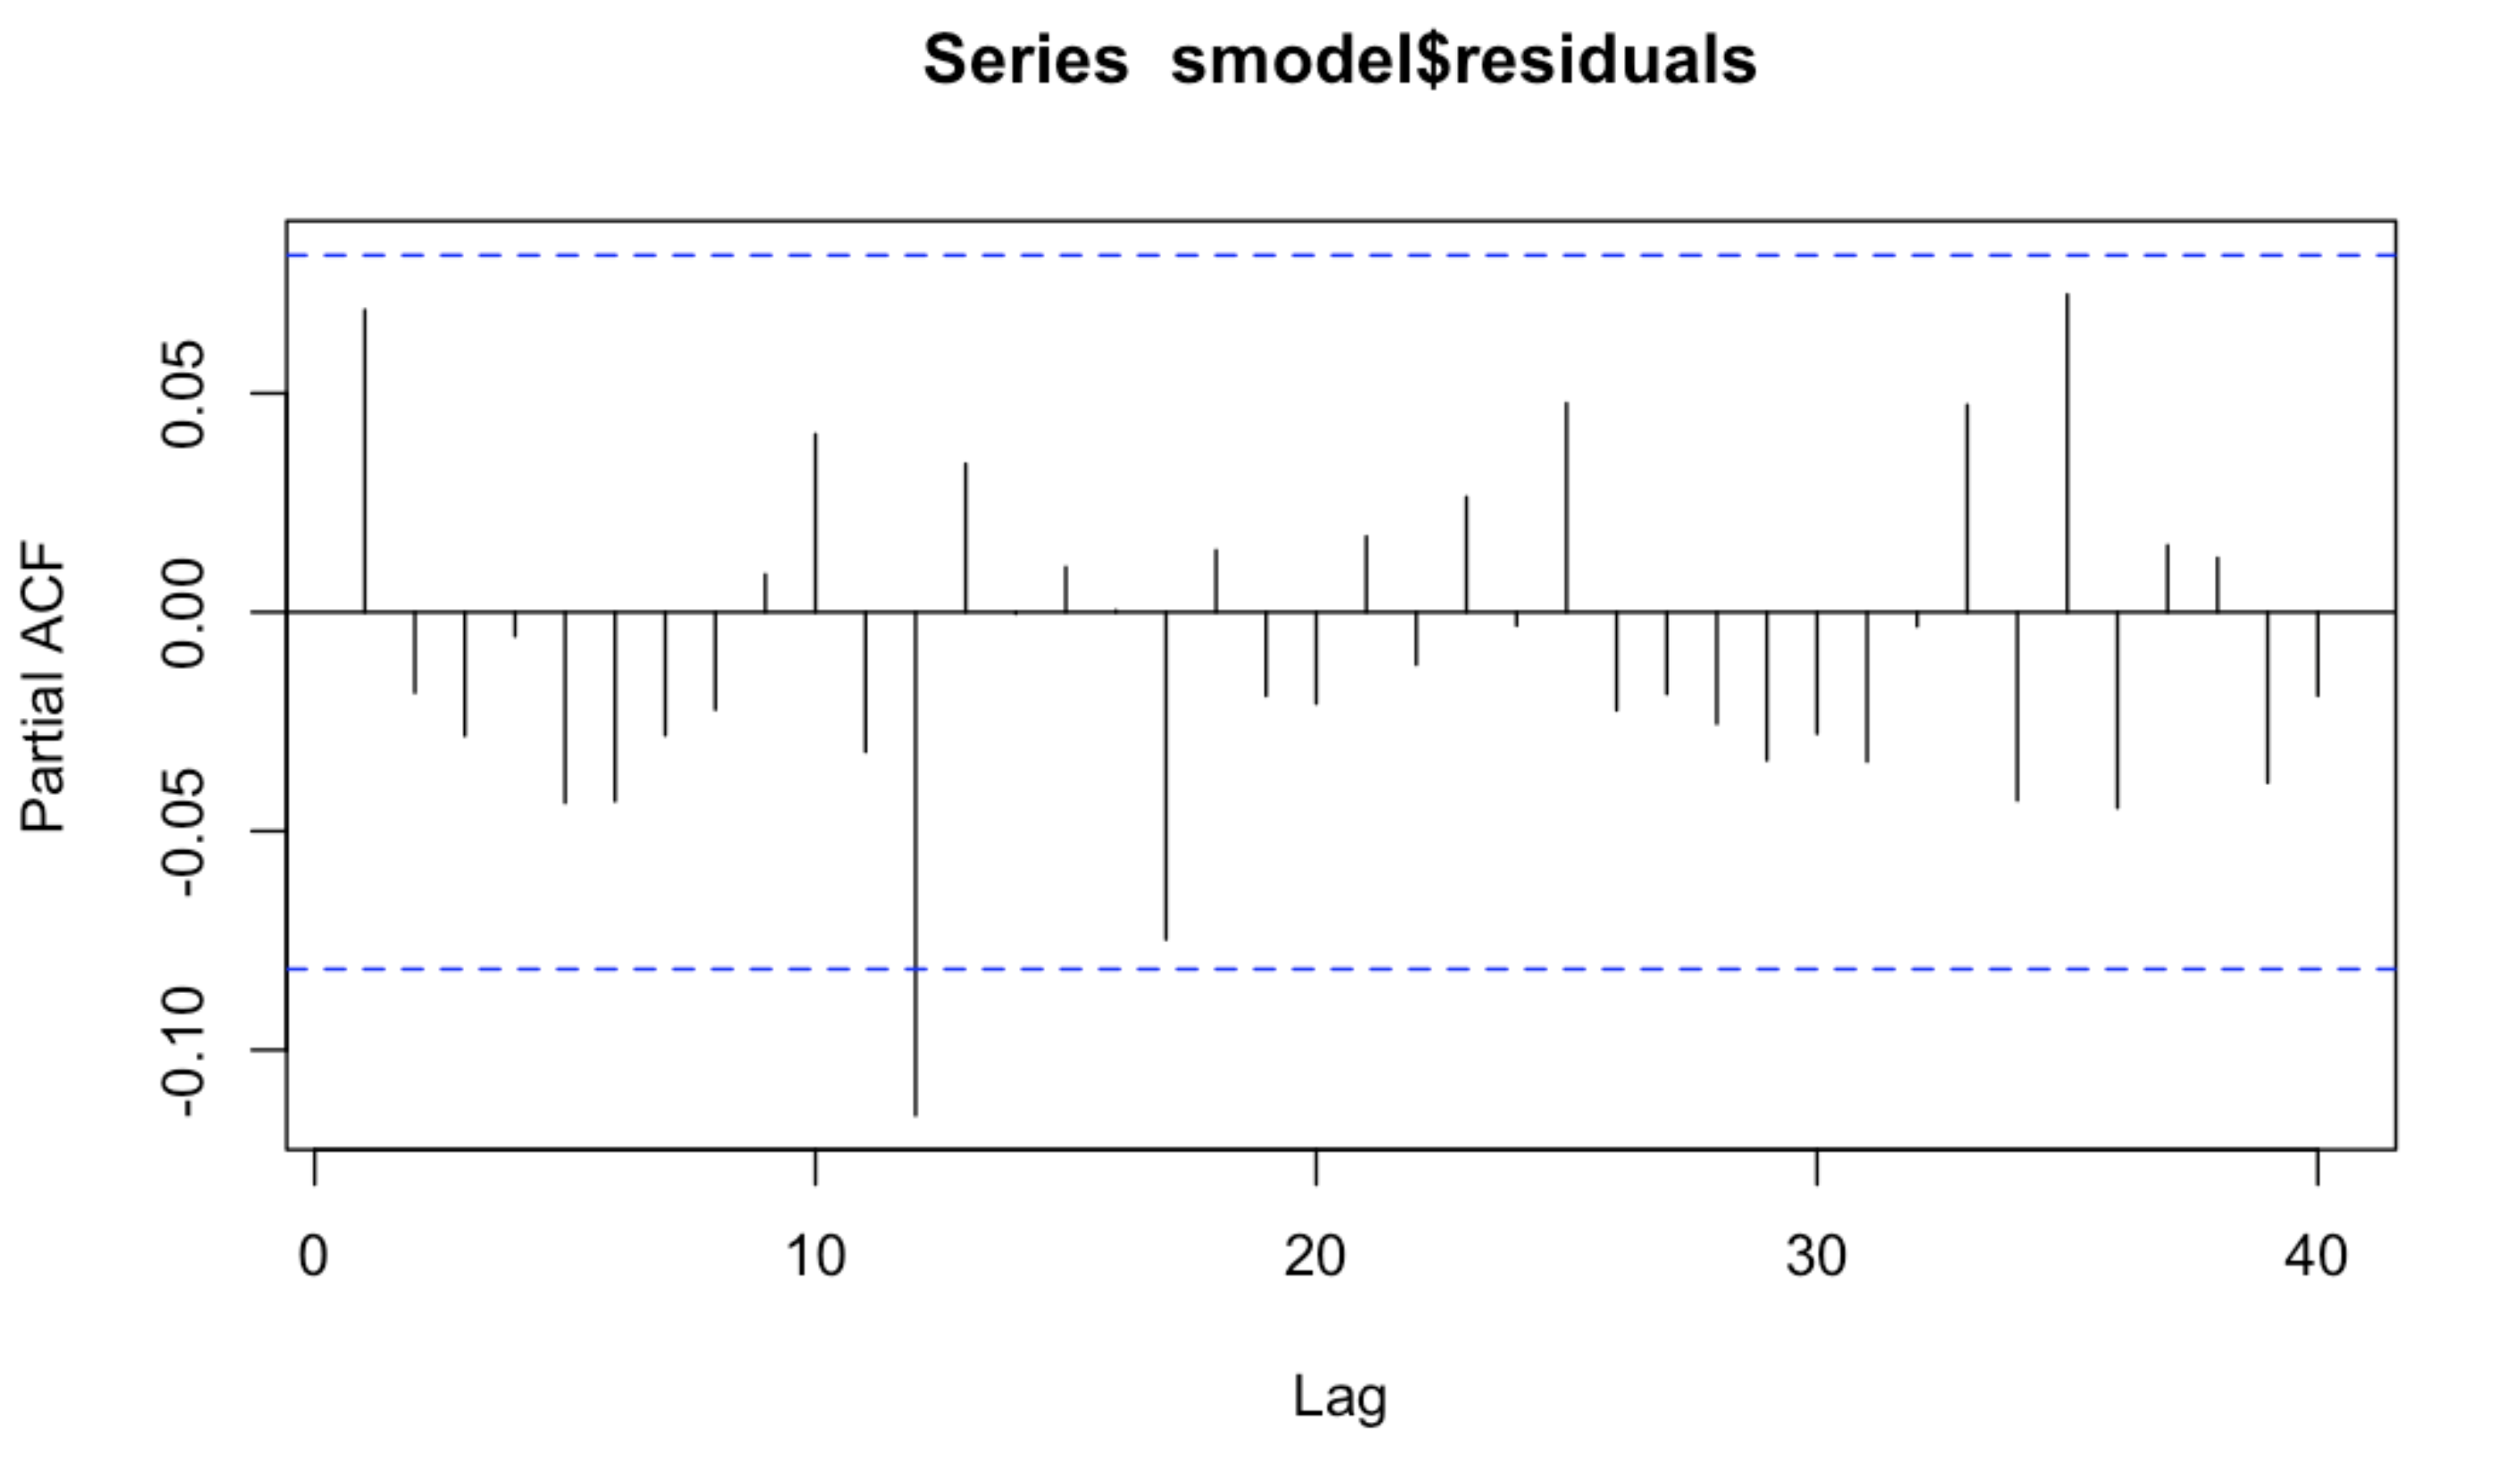
\includegraphics[width=0.7\textwidth]{ha-1_files/figure-markdown_strict/3-3-0-1.2.png}
        \label{fig:f8}
    \end{figure}

    \newpage
    \begin{figure}[H]
        \centering
        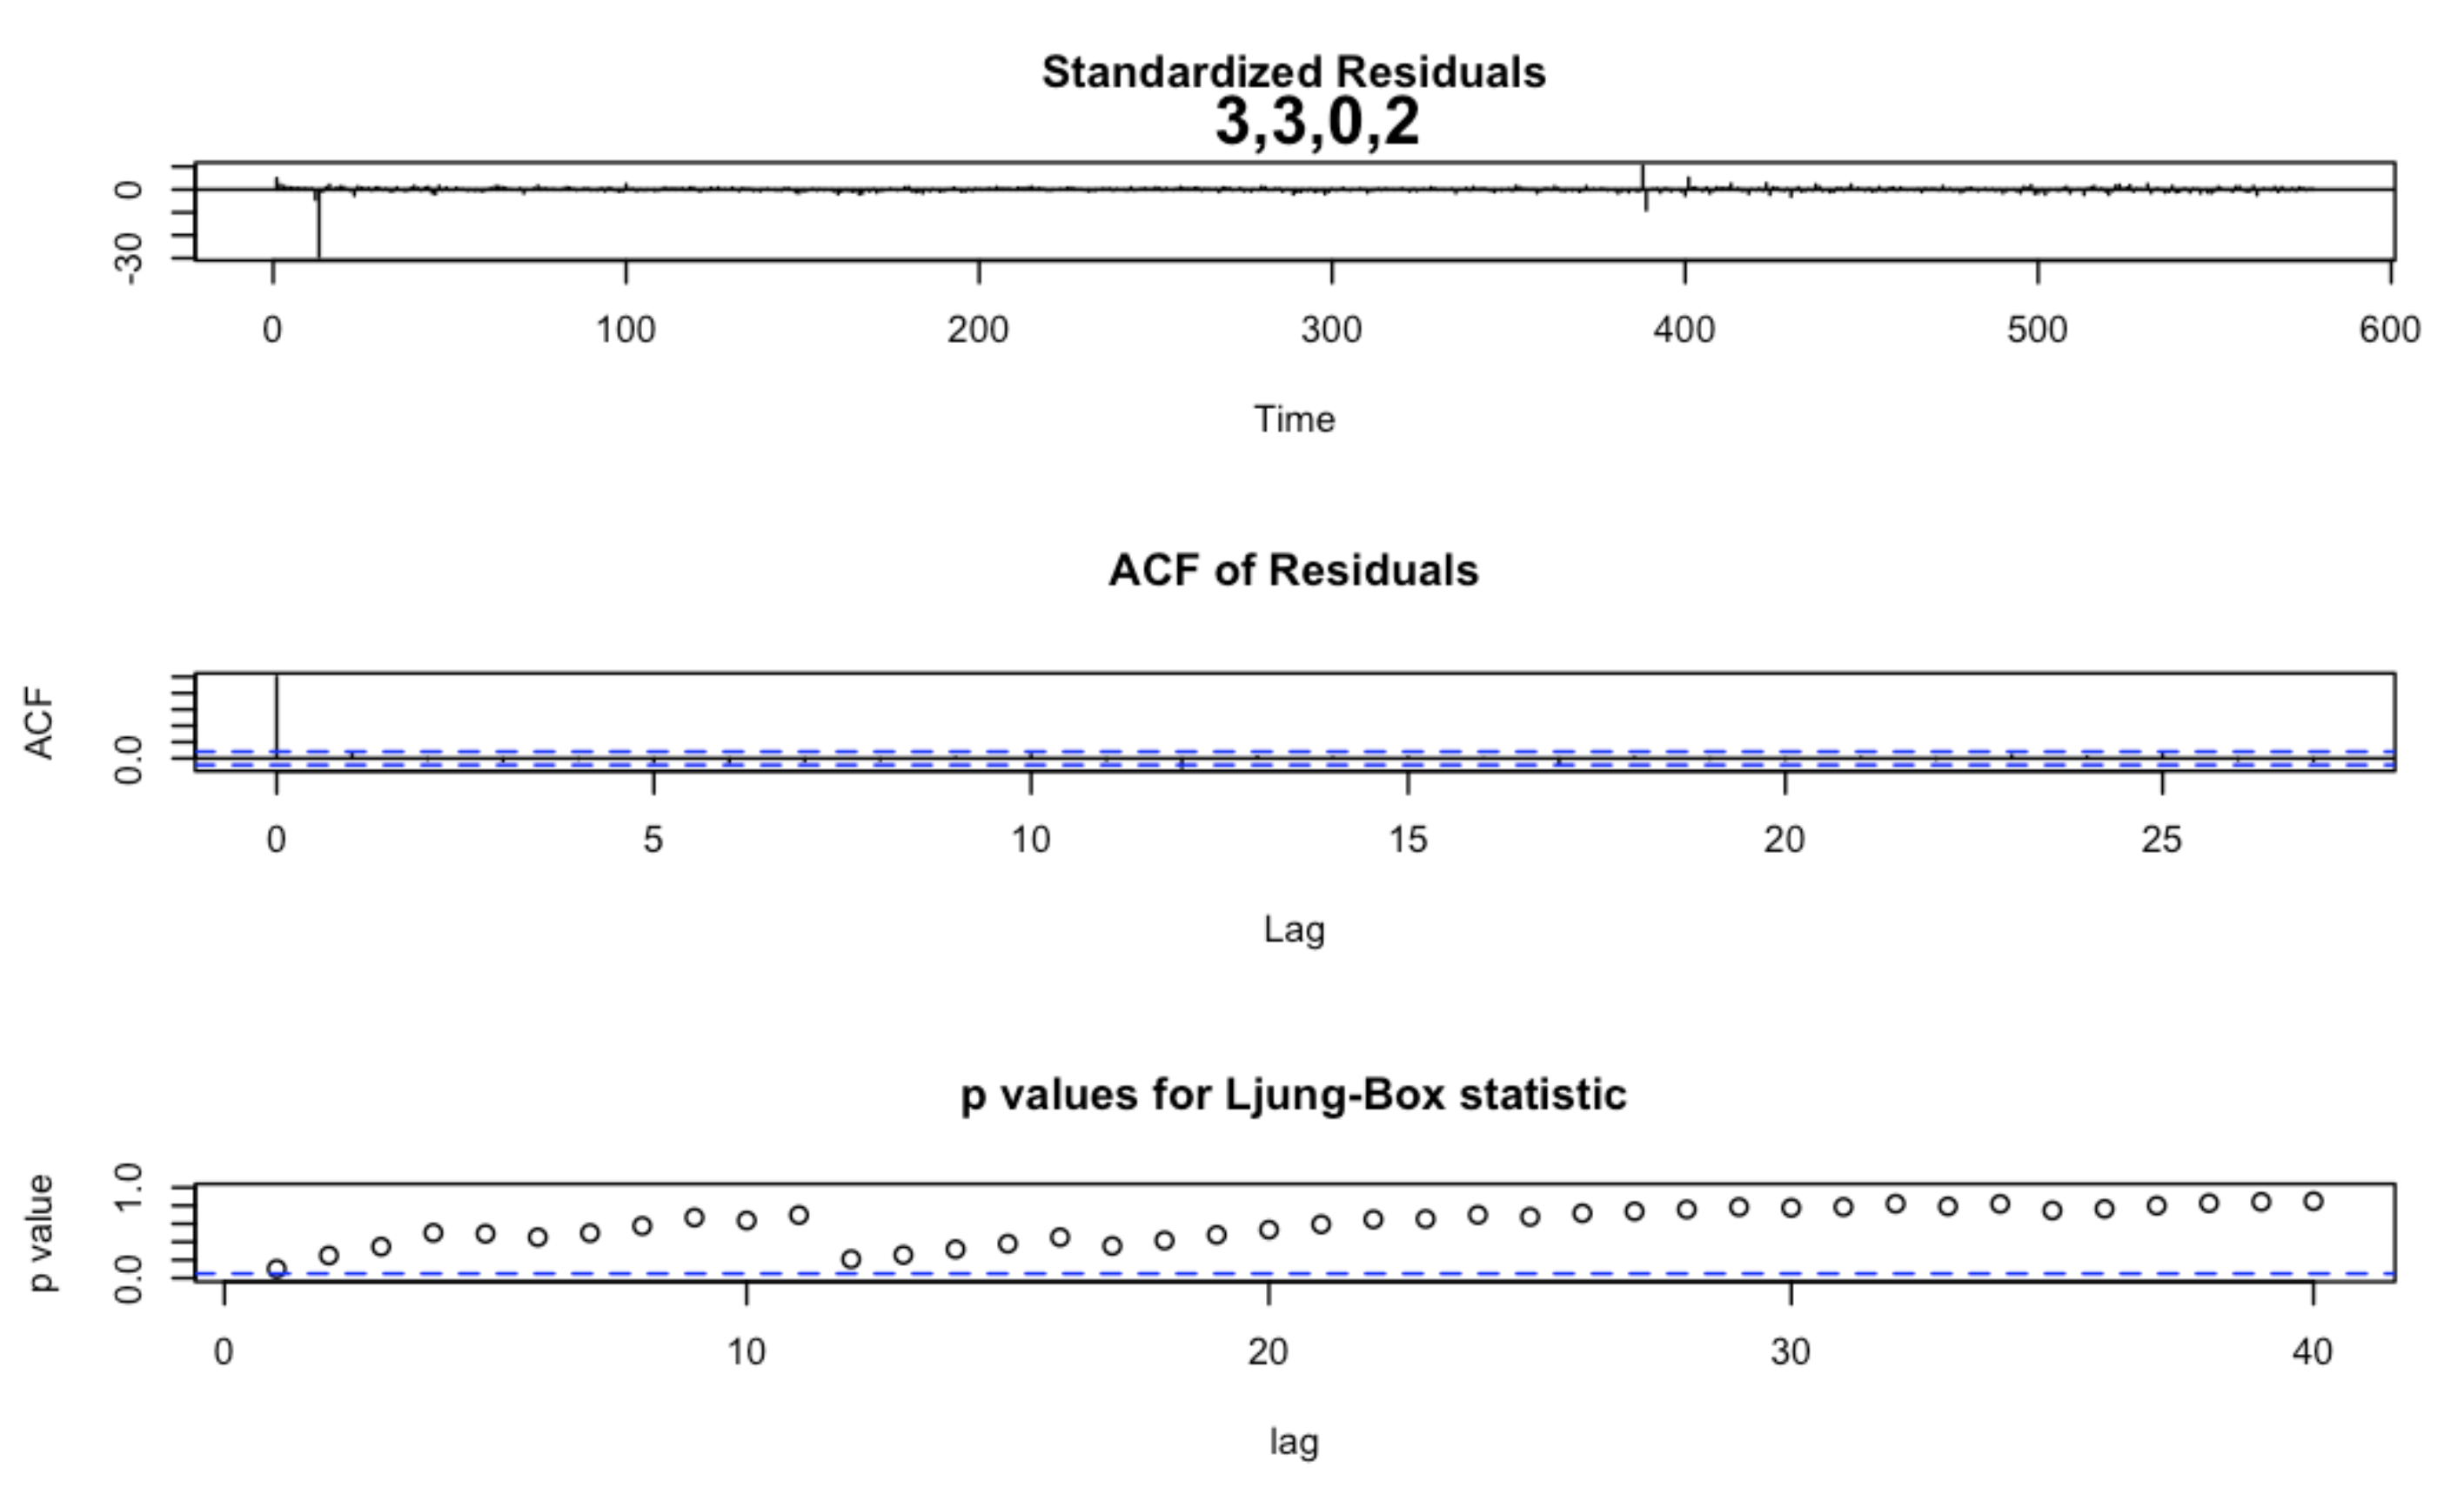
\includegraphics[width=0.7\textwidth]{ha-1_files/figure-markdown_strict/3-3-0-2.png}
        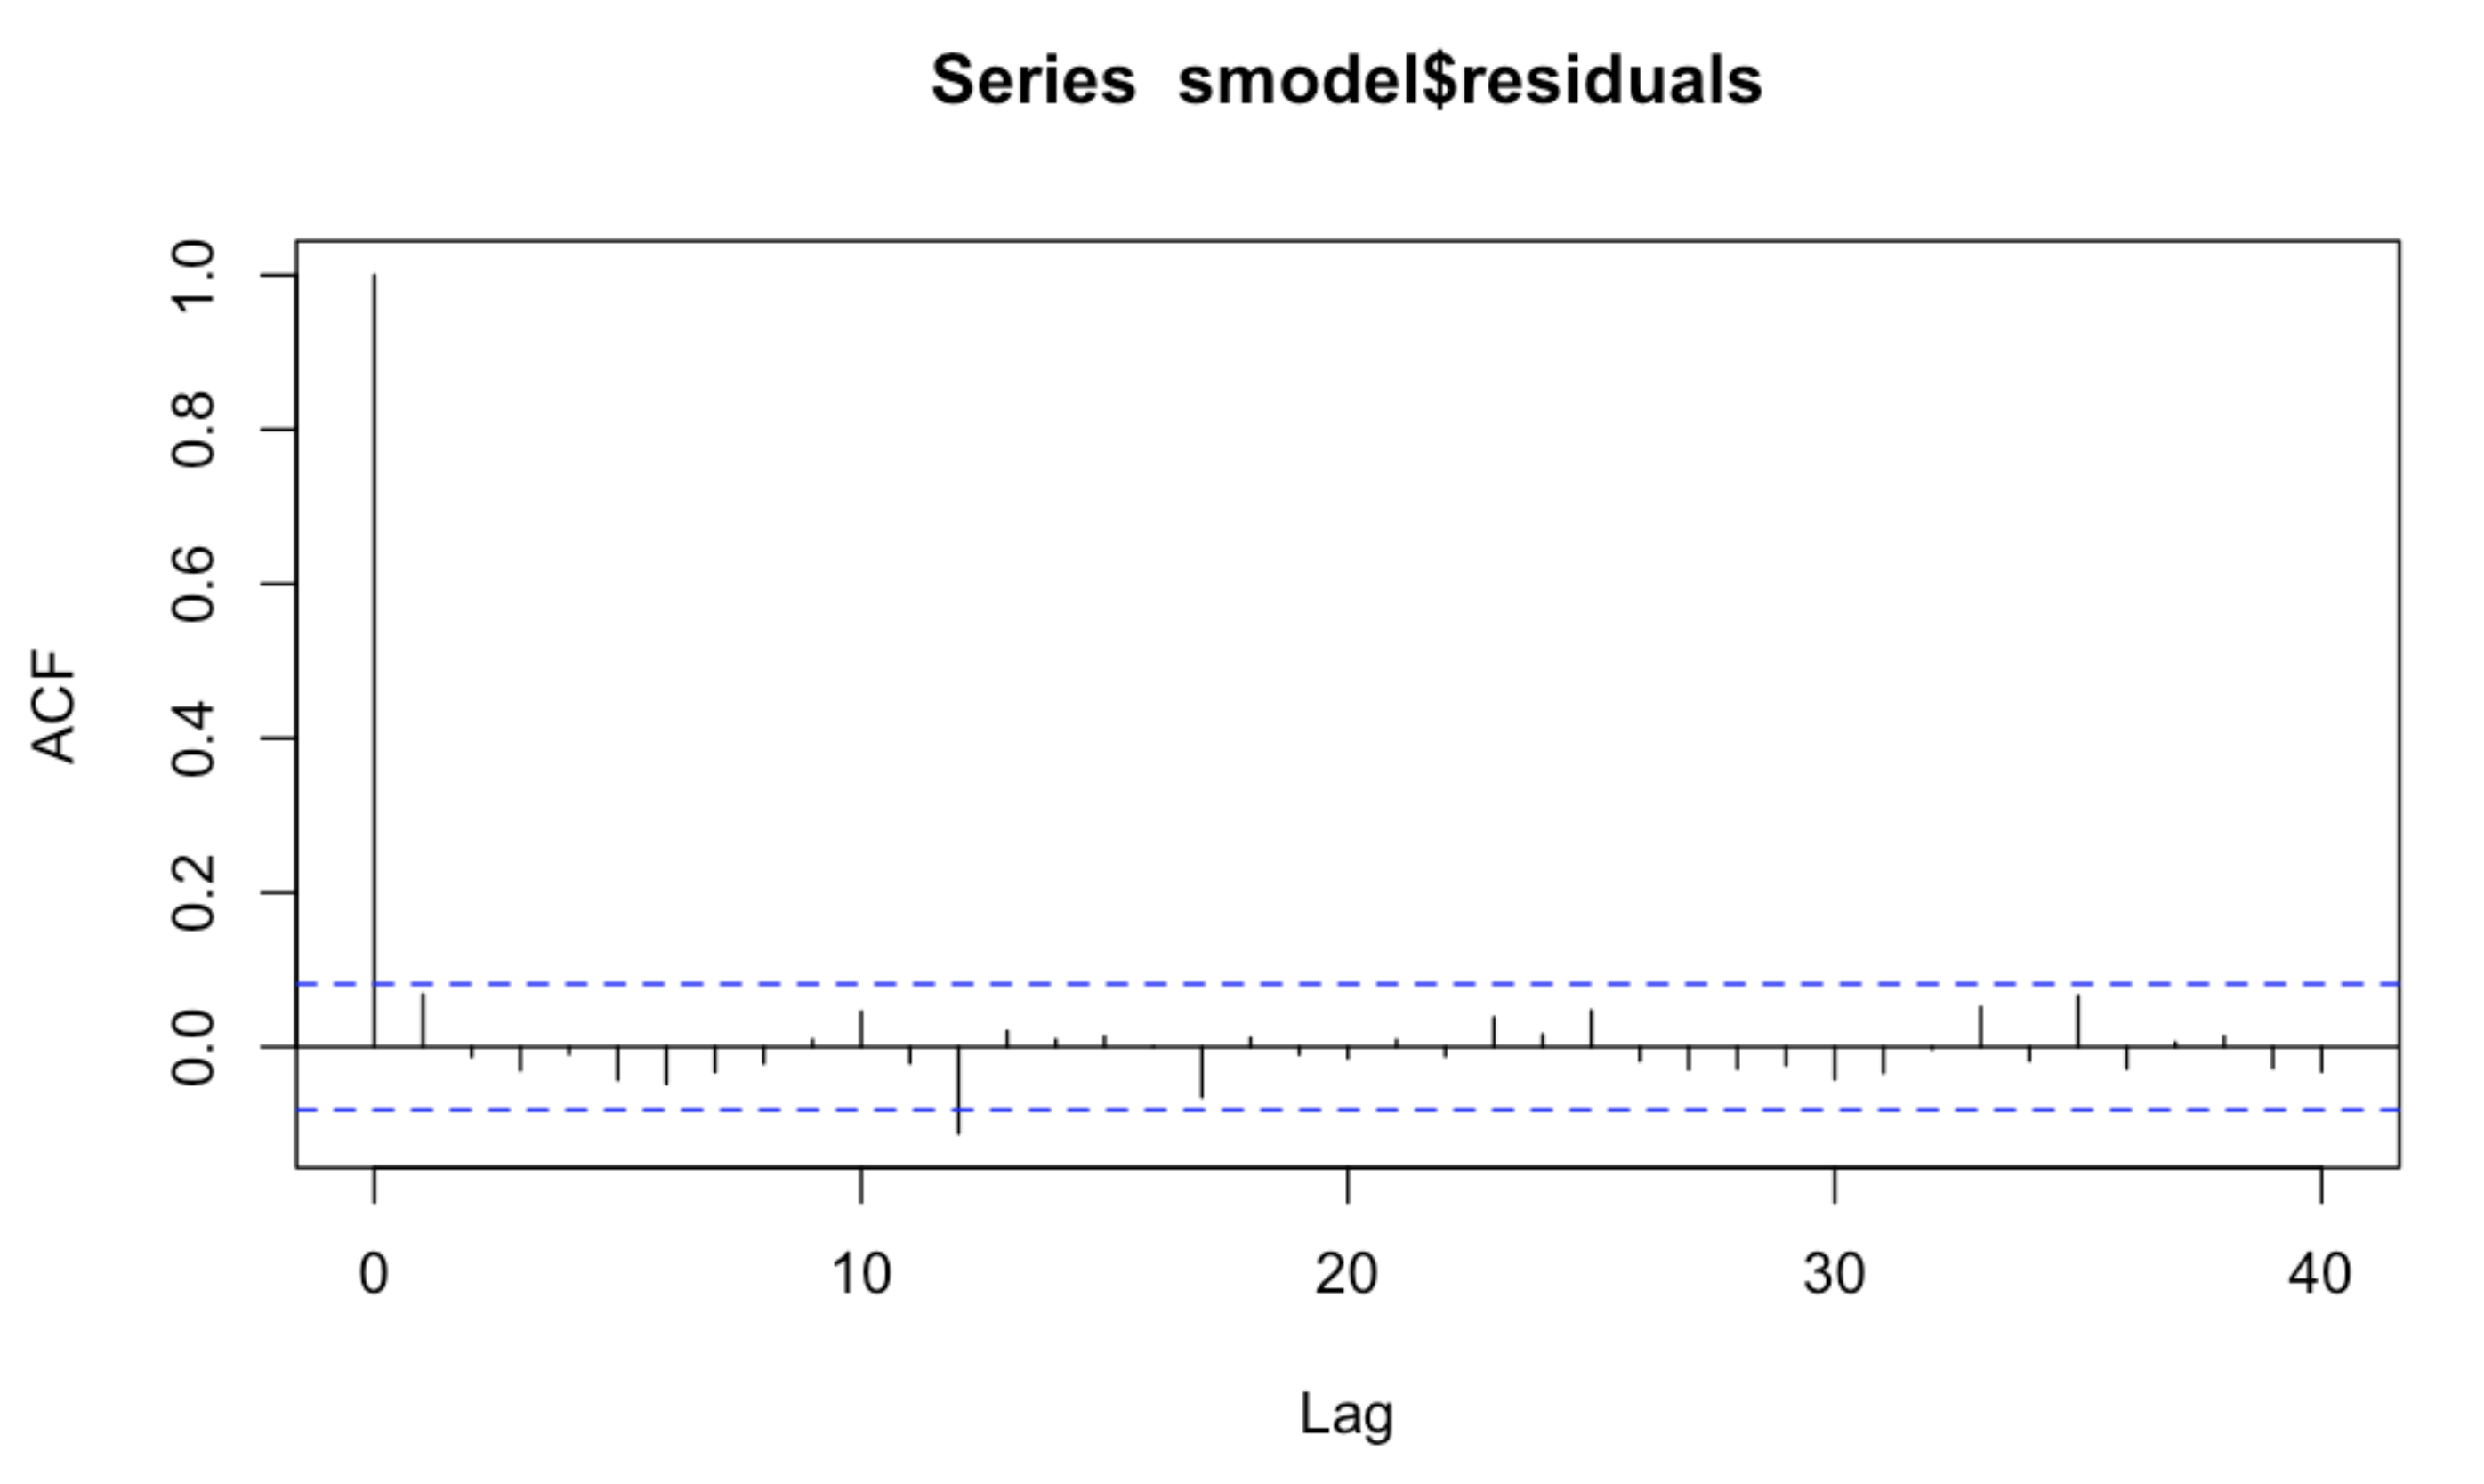
\includegraphics[width=0.7\textwidth]{ha-1_files/figure-markdown_strict/3-3-0-2.1.png}
        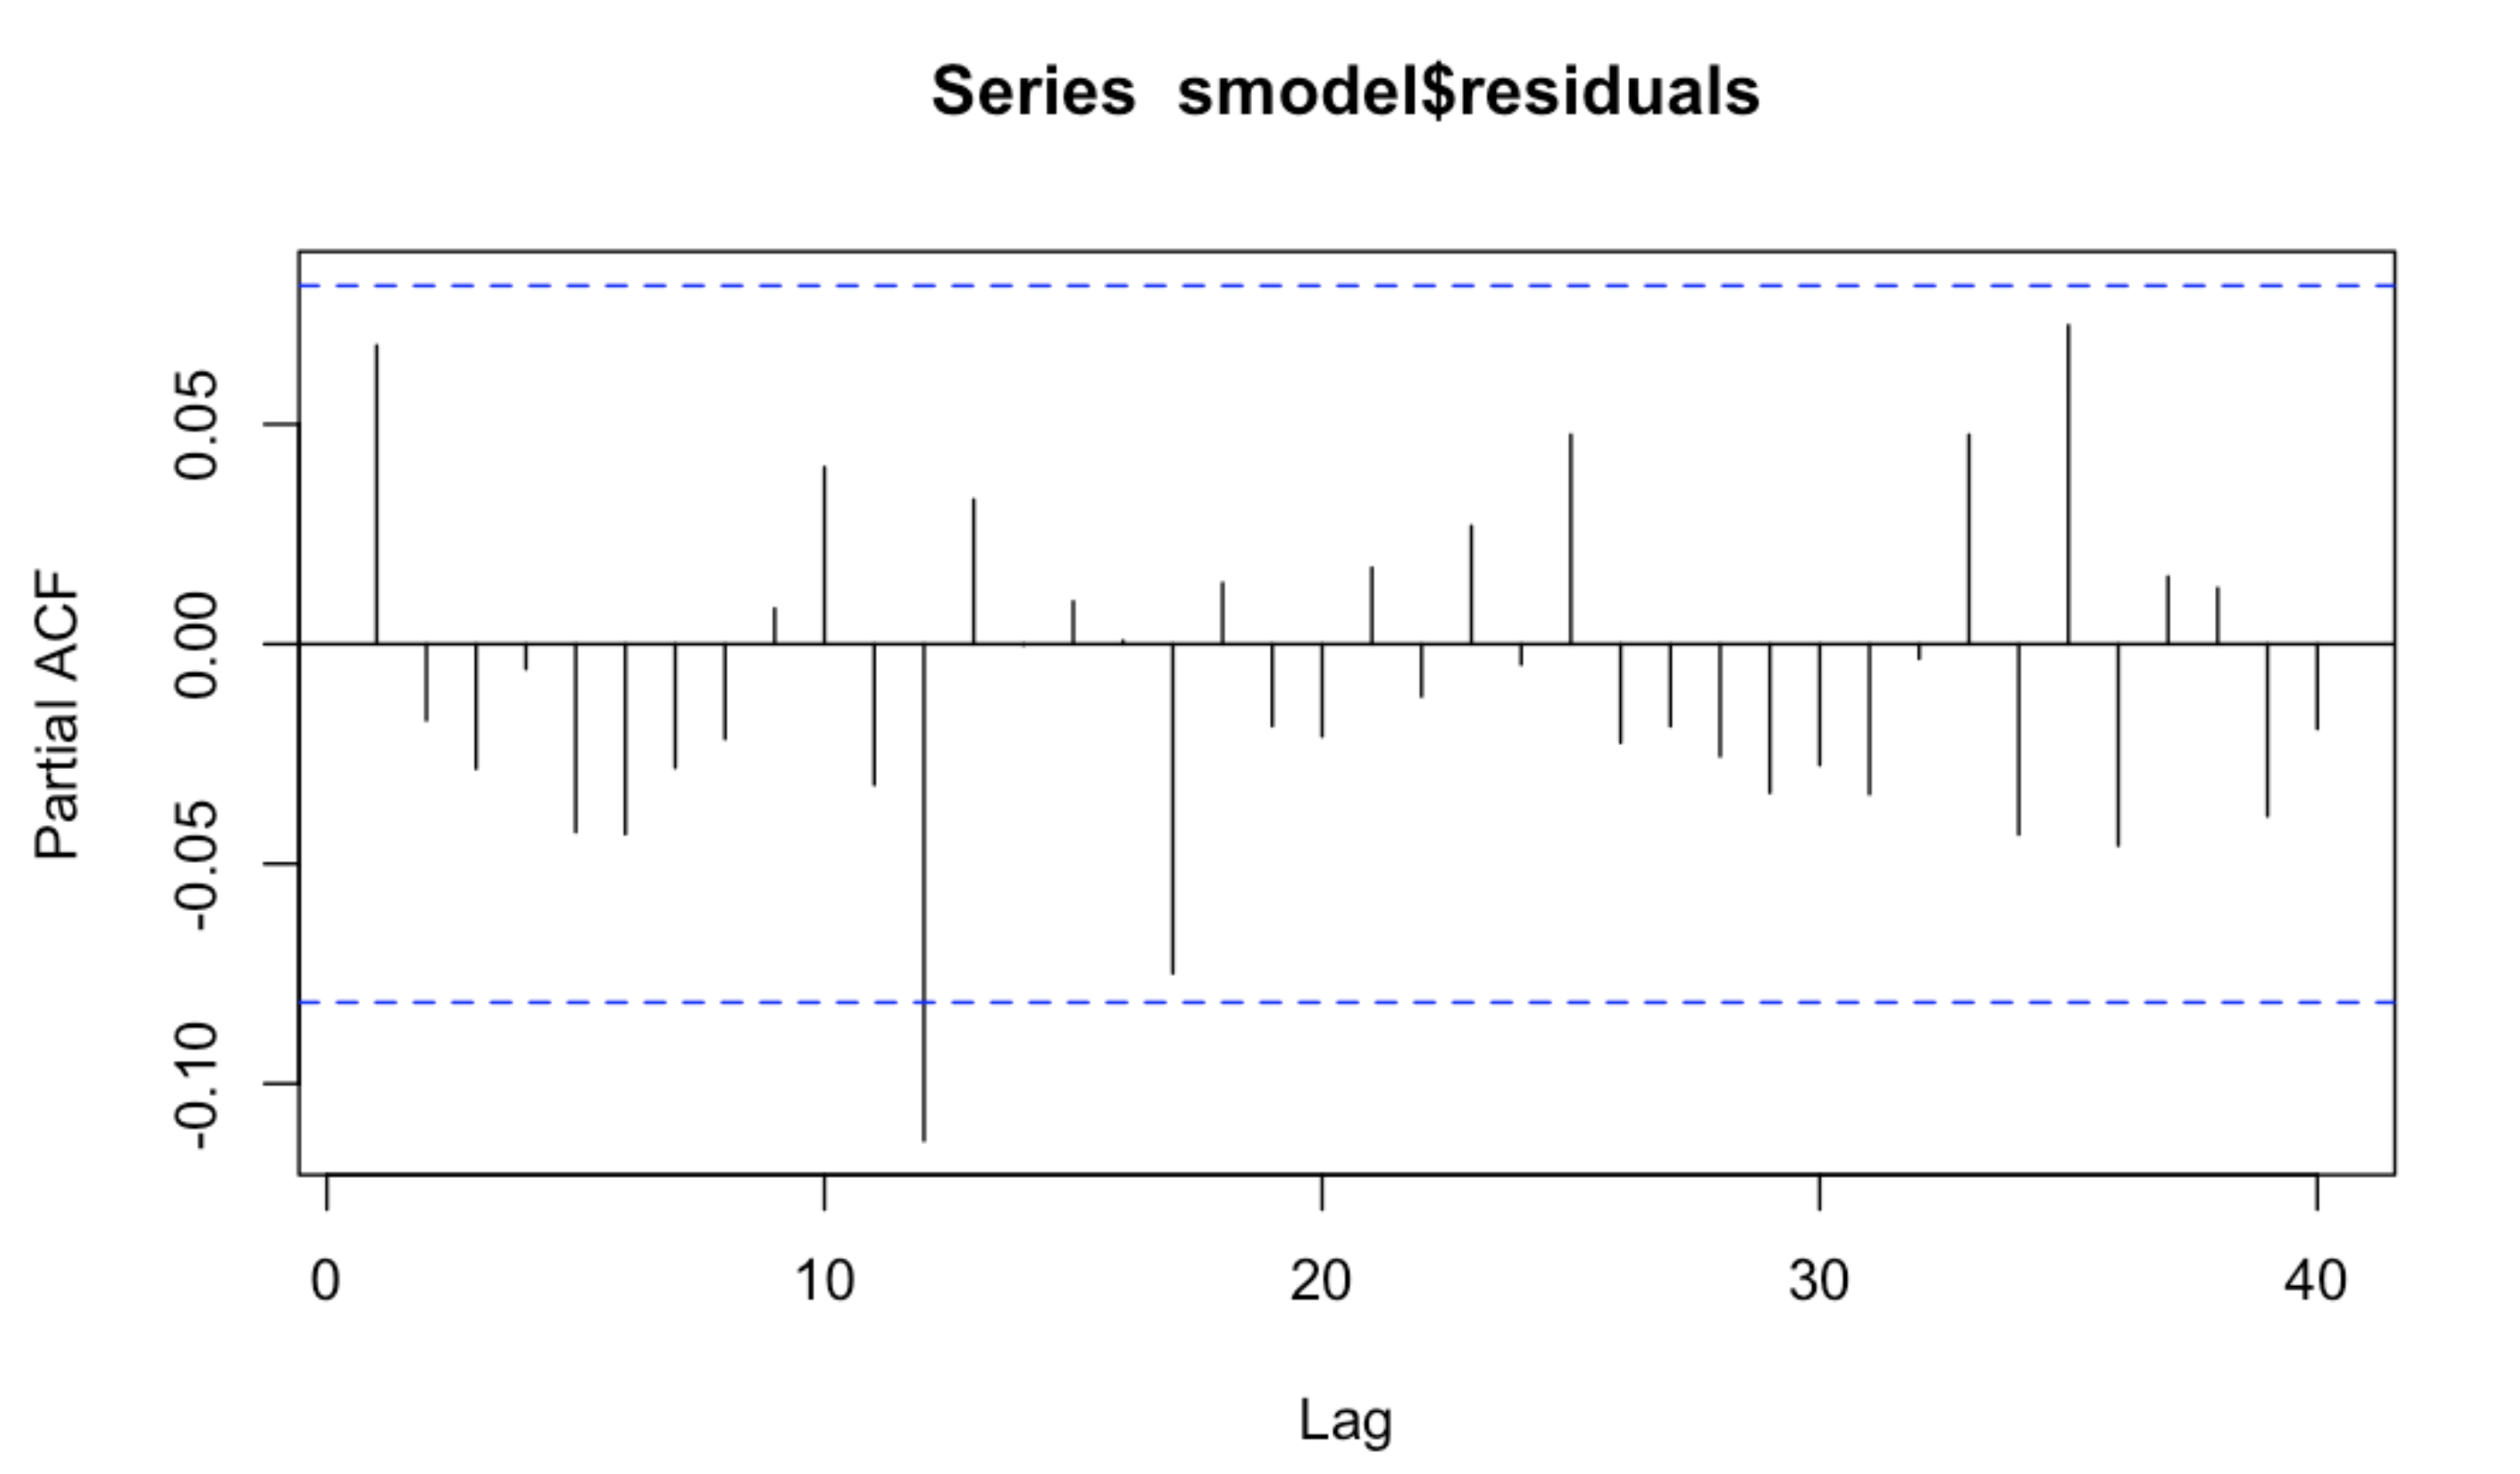
\includegraphics[width=0.7\textwidth]{ha-1_files/figure-markdown_strict/3-3-0-2.2.png}
        \label{fig:f9}
    \end{figure}

    \newpage
    \begin{figure}[H]
        \centering
        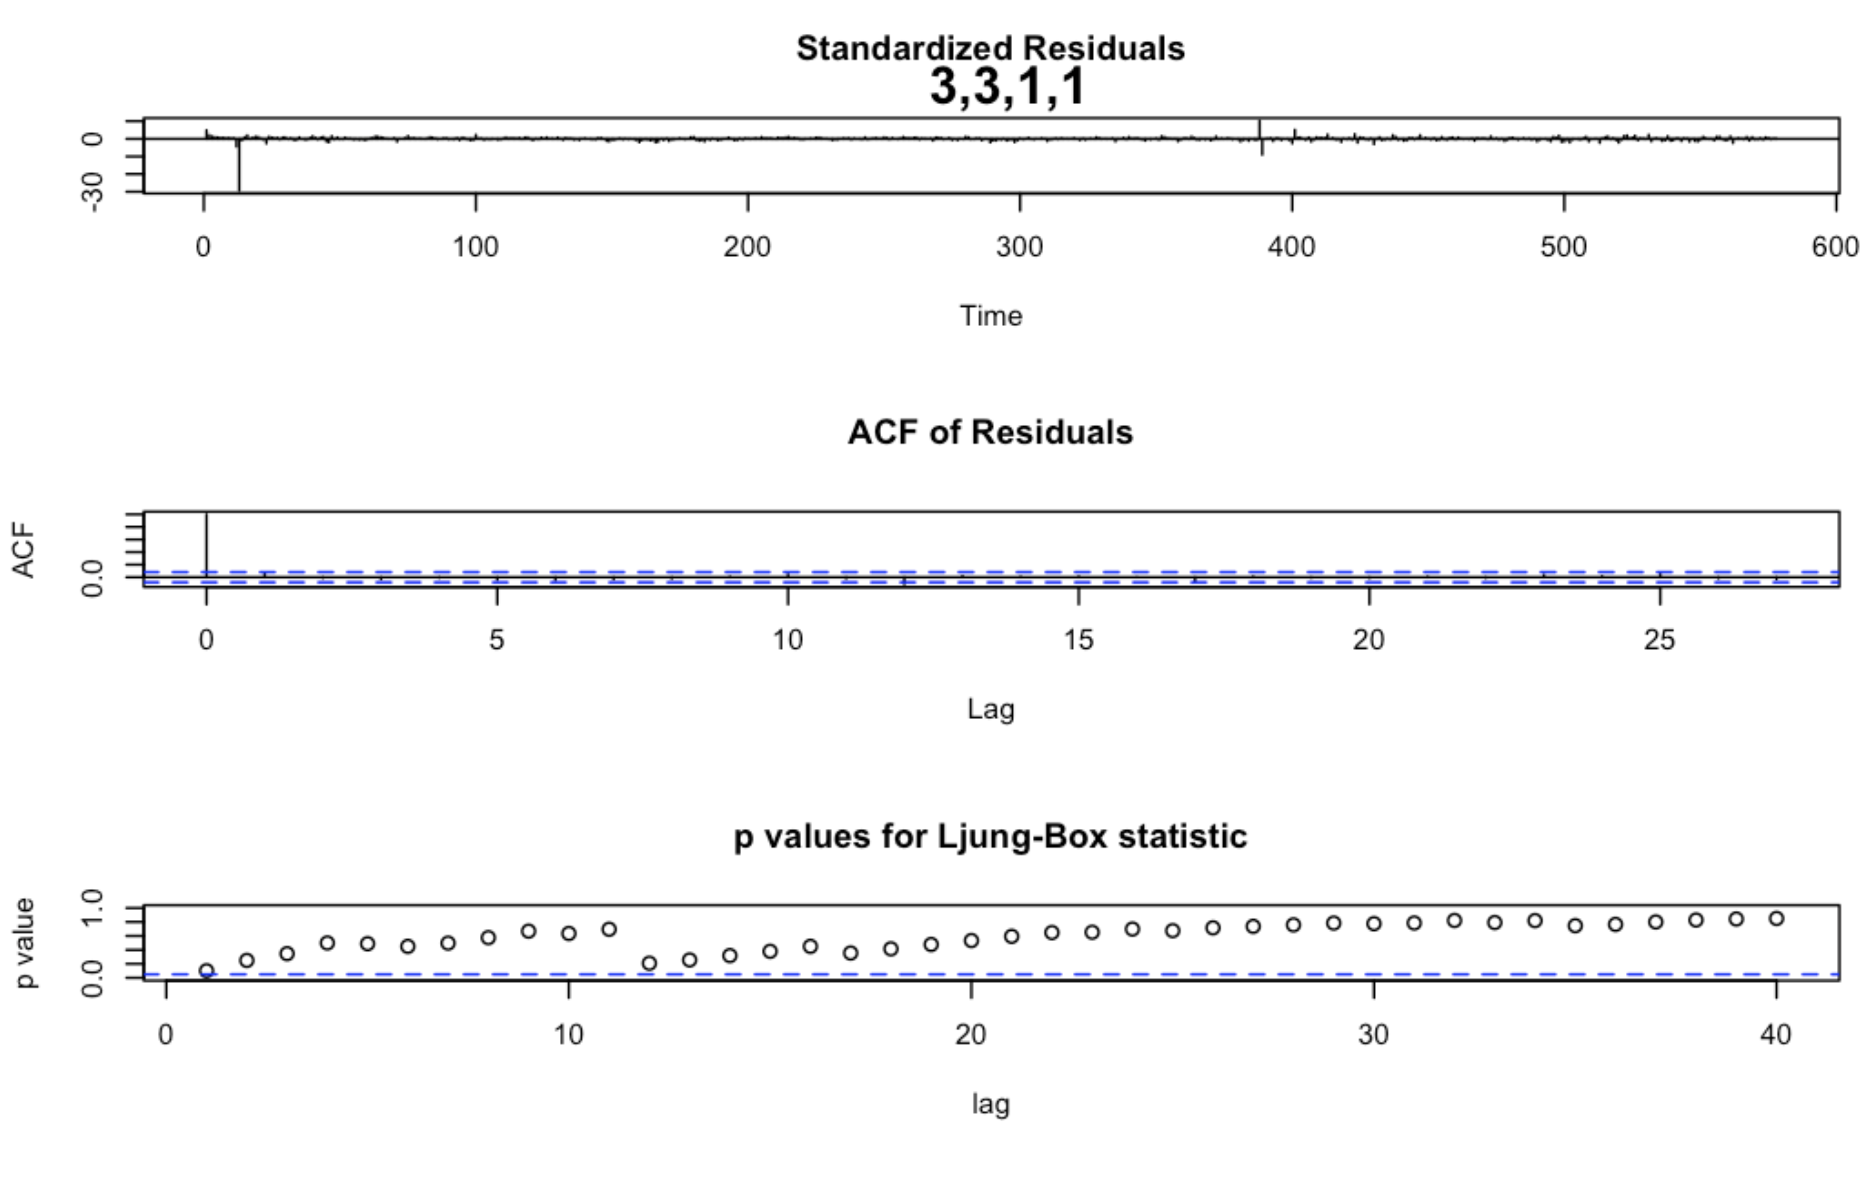
\includegraphics[width=0.7\textwidth]{ha-1_files/figure-markdown_strict/3-3-1-*.png}
        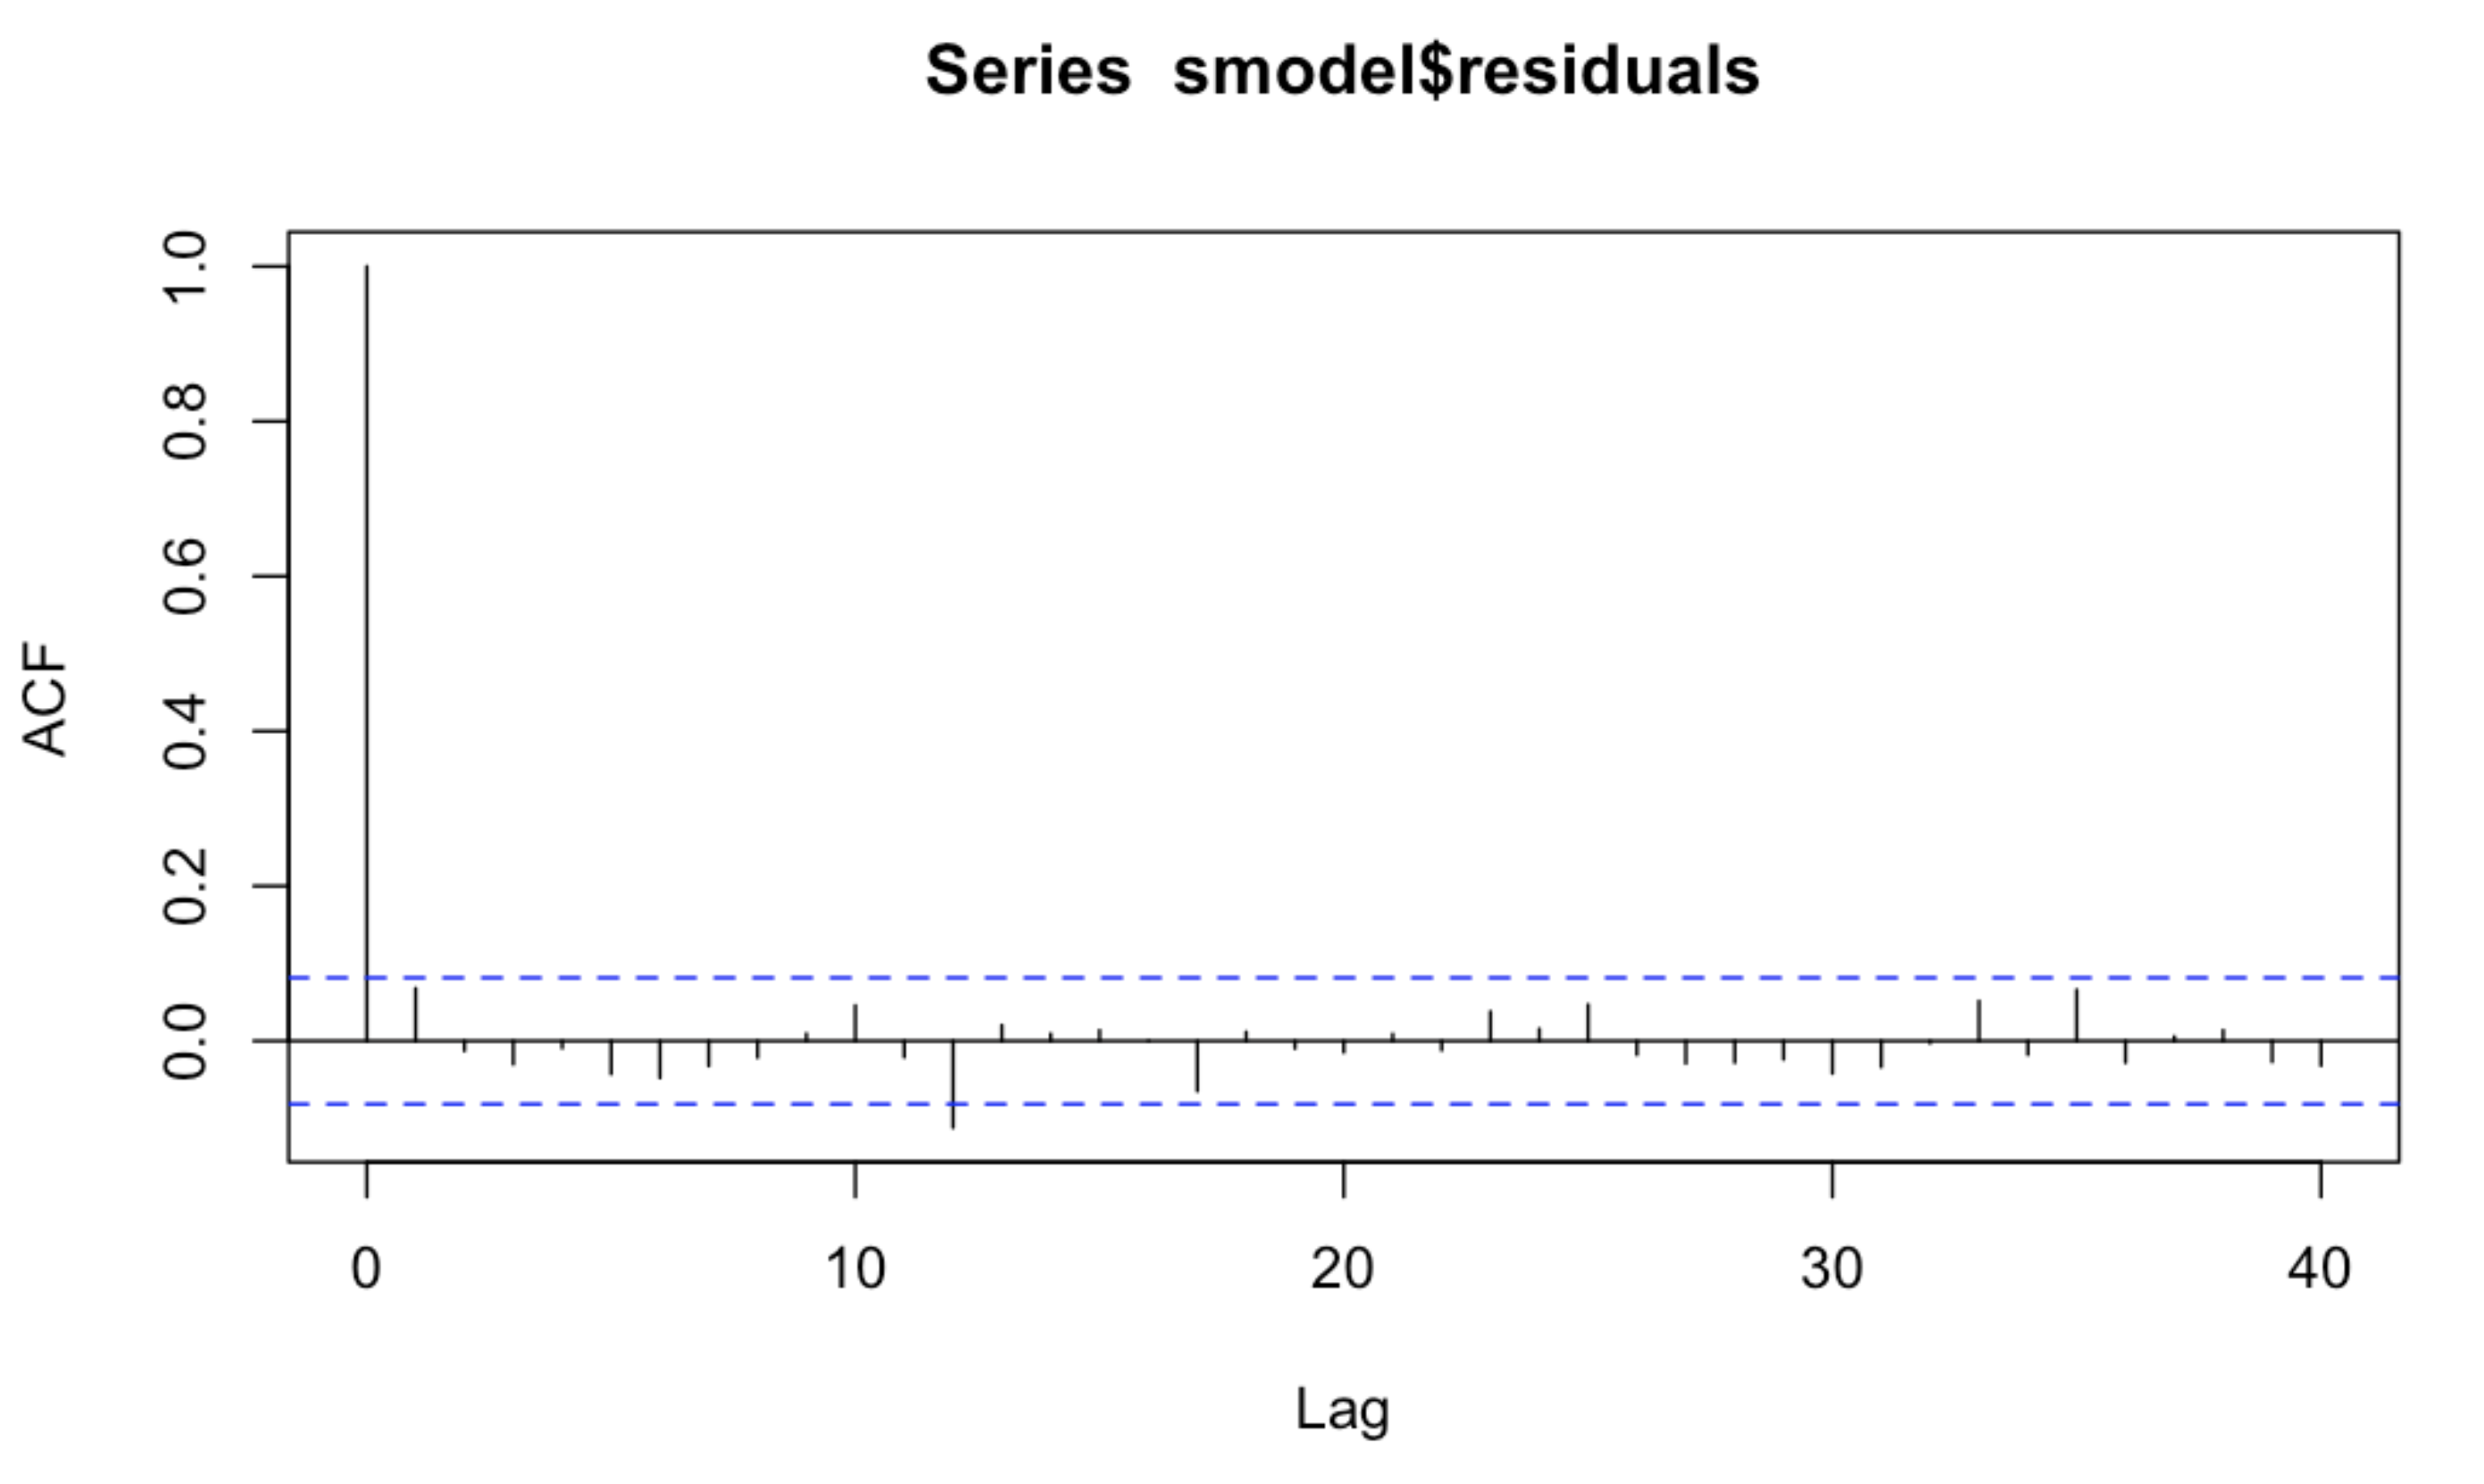
\includegraphics[width=0.7\textwidth]{ha-1_files/figure-markdown_strict/3-3-1-1.1.png}
        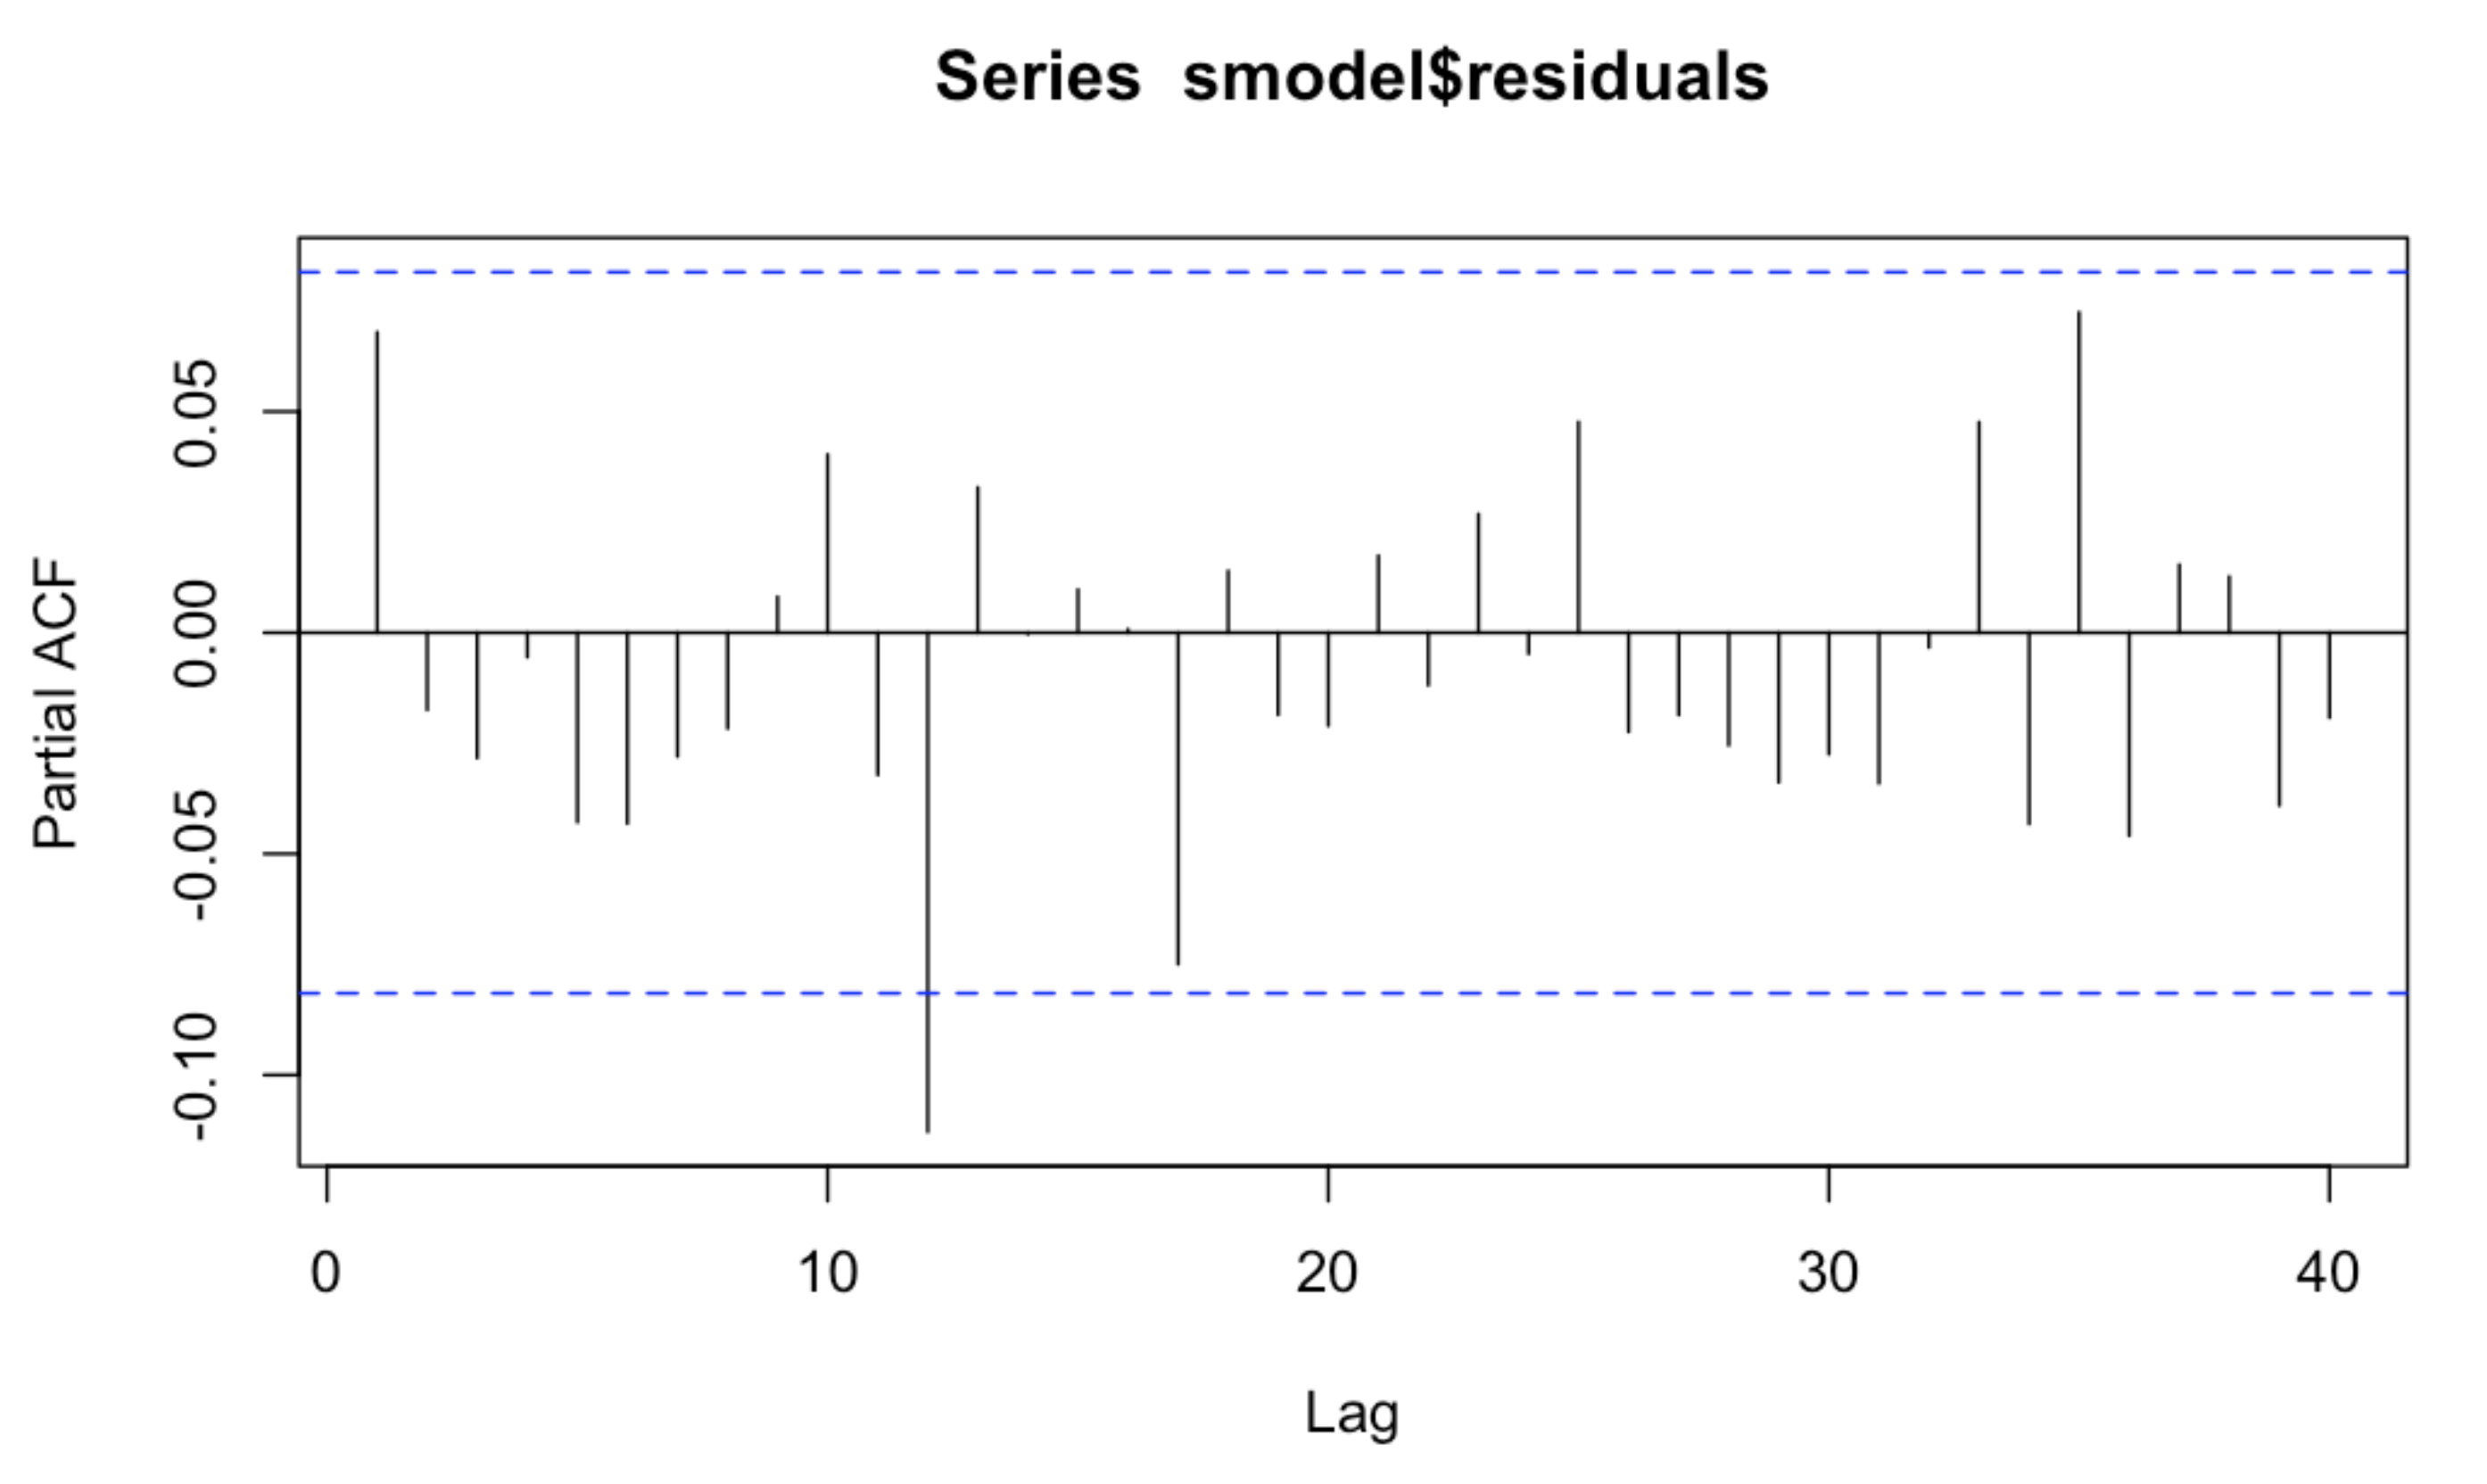
\includegraphics[width=0.7\textwidth]{ha-1_files/figure-markdown_strict/3-3-1-1.2.png}
        \label{fig:f10}
    \end{figure}

    \bibliographystyle{unsrt}
    \bibliography{references}

    \newpage
    \appendix
    \section{Code}
    \lstinputlisting[language=R, caption=R code used for Task 4.]{code.r}
\end{document}